\documentclass[en,11pt]{aghdpl}
%\documentclass[twoside]{aghdpl}
%\documentclass[pdflatex,en]{aghdpl}
\usepackage[english]{babel}
\usepackage[utf8]{inputenc}


\usepackage{enumerate}
\usepackage{enumitem}
\usepackage{listings}
\usepackage{hyperref}
\usepackage{fancyref}

\usepackage[titletoc,title]{appendix}
\usepackage[nottoc,numbib]{tocbibind}

\usepackage{graphicx}
\usepackage{caption}
\usepackage{subcaption}

\usepackage{todonotes}

\usepackage{listings}
% Scala listings
% "define" Scala
\lstdefinelanguage{scala}{
  morekeywords={abstract,case,catch,class,def,%%%%%%%%%%%%%%%%%%%%%%%%%%%%%%%%%%%%%%%%%%%%%%%%%%%%%%%%%%%%%%%%%%%%%%%%%%%%
% 
% File:     aghdpl.cls           (LaTeX Document class option "aghdpl")
%          
% Author:  Marcin Szpyrka     (mszpyrka@agh.edu.pl)
%          Grzegorz J. Nalepa (gjn@agh.edu.pl)
%          AGH University of Science and Technology, Kraków, POLAND
% 
%%%%%%%%%%%%%%%%%%%%%%%%%%%%%%%%%%%%%%%%%%%%%%%%%%%%%%%%%%%%%%%%%%%%%%%%%%%%

\message{*** [aghdpl.cls] ---  (MSz, GJN)  v0.22 <05.04.2011>  ***}       

\newif\ifpdflatex\pdflatexfalse
\NeedsTeXFormat{LaTeX2e} % 
\ProvidesClass{aghdpl} 
\DeclareOption{pdflatex}{\pdflatextrue}
\DeclareOption*{\PassOptionsToClass{\CurrentOption}{report}} 
\ProcessOptions\LoadClass[a4paper,oneside]{report} 

\RequirePackage{times}
\RequirePackage[T1]{fontenc}
\RequirePackage{graphicx}
\RequirePackage{geometry}
\RequirePackage[usenames]{color}
\RequirePackage{fancyhdr}
\RequirePackage{url}
\RequirePackage{titlesec}
\RequirePackage{tocloft}

\geometry{lmargin=30mm, rmargin=20mm, tmargin=20mm, bmargin=20mm, foot=10mm, head=10mm}
\definecolor{Green}{rgb}{0.1,0.5,0.1}

\def\shorttitlePL#1   {\gdef\@shorttitlePL{#1}}
\def\shorttitleEN#1   {\gdef\@shorttitleEN{#1}}
\def\shortauthor#1    {\gdef\@shortauthor{#1}}
\def\titlePL#1        {\gdef\@titlePL{#1}}
\def\titleEN#1        {\gdef\@titleEN{#1}}
\def\facultyEN#1      {\gdef\@facultyEN{#1}}
\def\facultyPL#1      {\gdef\@facultyPL{#1}}
\def\thesistypePL#1   {\gdef\@thesistypePL{#1}}
\def\thesistypeEN#1   {\gdef\@thesistypeEN{#1}}
\def\supervisorPL#1   {\gdef\@supervisorPL{#1}}
\def\supervisorEN#1   {\gdef\@supervisorEN{#1}}
\def\acknowledgements#1   {\gdef\@acknowledgements{#1}}
\def\departmentPL#1   {\gdef\@departmentPL{#1}}
\def\departmentEN#1   {\gdef\@departmentEN{#1}}

% \thesisheaders
% 
% \pagestyle{fancy}

%\bibliographystyle{abbrv}
\linespread{1.3}
\renewcommand{\labelitemi}{--}

%------------------------------------------------------------------------------

\newcommand{\titlepages}{%

\newpage \titlepage 

\begin{center}

\ifpdflatex
\includegraphics[scale=0.3]{agh}
\else
\includegraphics[scale=0.7]{agh}
\fi
\vspace*{1cm}


{\sffamily{\Large{\bfseries{\textsc Akademia G\'{o}rniczo-Hutnicza im. Stanis\l{}awa Staszica w Krakowie}}}\\
{\Large\bfseries{\textsc{{Wydzia\l{} Elektrotechniki, Automatyki,}\\ {Informatyki i In\.zynierii Biomedycznej}}}}}\\\vspace*{2mm}
{\Large\textsc{\@departmentPL}}\\\vspace*{1.5cm}


{\LARGE\@thesistypePL}\\\vspace*{1.5cm}

{\huge{\emph{Przetwarzanie i analiza danych multimedialnych\\ w \'{s}rodowisku rozproszonym}}}\\\vspace*{1cm}
{\huge{\emph{Processing and analisys of multimedia \\in distributed systems}}}\\\vspace*{2.5cm}

\begin{flushleft}
\begin{minipage}[!h]{12cm} 
\Large{ Autor: \@author}\\ 
\Large{ Kierunek studi\'{o}w: Informatyka}\\ 
\Large{ Opiekun pracy: \@supervisorPL}\\ 
\end{minipage}
\end{flushleft}

\vfill
{\large Krak\'{o}w, \@date}

\end{center}

\clearpage \titlepage 

\begin{flushleft}
\begin{minipage}[!h]{10.5cm}
\emph{ O\'swiadczam, \'swiadomy odpowiedzialno\'sci karnej za po\'swiadczenie nieprawdy, \.ze niniejsz\k{a} prac\k{e} dyplomow\k{a} wykona\l{}em osobi\'scie i~samodzielnie, i nie korzysta\l{}em ze \'zr\'ode\l{} innych ni\.z wymienione w~pracy.}\\
\end{minipage}

\vspace{1cm}

\makebox[6cm][s]{\dotfill}\par
\makebox[6cm][c]{\small PODPIS}

\end{flushleft}
\vfill
\clearpage \titlepage

\vspace*{15cm} \vfill
\begin{flushright} 
\begin{minipage}[!h]{10cm}
{\Large \@acknowledgements}
\end{minipage}
\end{flushright}

\clearpage

\setcounter{page}{5}

}

\def\thesisheaders{
\fancyfoot[L]{\small \@shortauthor\quad\textit{\@shorttitlePL}}
}

\DeclareOption{en}{
\def\thesisheaders{
\fancyfoot[L]{\small \@shortauthor\quad\textit{\@shorttitleEN}}
}
}

\ProcessOptions

\pagestyle{fancy}
\renewcommand{\chaptermark}[1]{\markboth{\thechapter.\ #1}{}}
\renewcommand{\sectionmark}[1]{\markright{\thesection.\ #1}}
\renewcommand{\headrulewidth}{0.5pt}
\renewcommand{\footrulewidth}{0.5pt}
\fancyhf{}
\fancyhead{}
\fancyhead[RE]{\slshape{\small \rightmark}}
\fancyhead[LE]{\bfseries \thepage}
\fancyhead[LO]{\slshape{\small \rightmark}}
\fancyhead[RO]{\bfseries \thepage}

\thesisheaders

\frenchspacing
\sloppy 
\widowpenalty     9999 
\clubpenalty      9999 
\flushbottom

%---------------------------------------------------------------------------
% Ustawienia parametrów dla tytu³ów rozdzia³ów, podrozdzia³ów, itd.
%---------------------------------------------------------------------------


\titleformat{\chapter}[block]
{\bfseries\LARGE}{\filright \LARGE\thechapter. }{0ex}{}
%odstêpy: lewy, góra, dó³
\titlespacing{\chapter}{0pt}{17mm}{19mm}
\titleformat{\section}[block]
{\bfseries\Large}{\filright \Large\thesection. }{0ex}{}
\titlespacing{\section}{7mm}{8mm plus 0mm minus 1mm}{4mm plus 0mm minus 1mm}
\titleformat{\subsection}[block]
{\bfseries\large}{\filright \large\thesubsection. }{0ex}{}
\titlespacing{\subsection}{7mm}{6mm}{2.5mm}
\titleformat{\subsubsection}[block]
{\bfseries\normalsize}{\filright \normalsize\thesubsubsection. }{0ex}{}
\titlespacing{\subsubsection}{7mm}{3mm}{1.5mm}

%---------------------------------------------------------------------------
% Ustawienia parametrów generowania spisu tre¶ci i spisu rysunków
%---------------------------------------------------------------------------

\renewcommand{\cfttoctitlefont}{\bfseries\Large}
\renewcommand{\cftbeforetoctitleskip}{20mm}
\renewcommand{\cftaftertoctitleskip}{19mm}
\renewcommand{\cftchapleader}{\cftdotfill{\cftdot}}
\renewcommand{\cftsecleader}{\cftdotfill{\cftdot}}
\renewcommand{\cftsubsecleader}{\cftdotfill{\cftdot}}
\renewcommand{\cftchapaftersnum}{.}
\renewcommand{\cftsecaftersnum}{.}
\renewcommand{\cftsubsecaftersnum}{.}
\setlength{\cftparskip}{2pt}
\setlength{\cftbeforechapskip}{0mm}
\renewcommand{\cftchappagefont}{\normalsize}

    do,else,extends,false,final,finally,%
    for,if,implicit,import,match,mixin,%
    new,null,object,override,package,%
    private,protected,requires,return,sealed,%
    super,this,throw,trait,true,try,%
    type,val,var,while,with,yield},
  otherkeywords={=>,<-,<\%,<:,>:,\#,@},
  sensitive=true,
  morecomment=[l]{//},
  morecomment=[n]{/*}{*/},
  morestring=[b]",
  morestring=[b]""",
  morestring=[s][\color{blue}]{'}{a},
  morestring=[s][\color{blue}]{'}{d}
}

% IntelliJ Colors for listings
\usepackage{color}
\definecolor{dkgreen}{rgb}{0,0.6,0}
\definecolor{gray}{rgb}{0.5,0.5,0.5}
\definecolor{mauve}{rgb}{0.58,0,0.82}
 
% Default settings for code listings
\lstset{
  frame=tb,
  language=Scala,
  aboveskip=3mm,
  belowskip=3mm,
  showstringspaces=false,
  columns=flexible,
  basicstyle={\small\ttfamily},
  numbers=left,
  numberstyle=\small\color{gray},
  keywordstyle=\color{blue},
  commentstyle=\color{gray},
  stringstyle=\color{dkgreen},
  frame=single,
  breaklines=true,
  breakatwhitespace=true
  tabsize=2
}

\lstloadlanguages{TeX}

\lstset{
  literate={ą}{{\k{a}}}1
           {ć}{{\'c}}1
           {ę}{{\k{e}}}1
           {ó}{{\'o}}1
           {ń}{{\'n}}1
           {ł}{{\l{}}}1
           {ś}{{\'s}}1
           {ź}{{\'z}}1
           {ż}{{\.z}}1
           {Ą}{{\k{A}}}1
           {Ć}{{\'C}}1
           {Ę}{{\k{E}}}1
           {Ó}{{\'O}}1
           {Ń}{{\'N}}1
           {Ł}{{\L{}}}1
           {Ś}{{\'S}}1
           {Ź}{{\'Z}}1
           {Ż}{{\.Z}}1
}


\lstset{
  literate={ą}{{\k{a}}}1
           {ć}{{\'c}}1
           {ę}{{\k{e}}}1
           {ó}{{\'o}}1
           {ń}{{\'n}}1
           {ł}{{\l{}}}1
           {ś}{{\'s}}1
           {ź}{{\'z}}1
           {ż}{{\.z}}1
           {Ą}{{\k{A}}}1
           {Ć}{{\'C}}1
           {Ę}{{\k{E}}}1
           {Ó}{{\'O}}1
           {Ń}{{\'N}}1
           {Ł}{{\L{}}}1
           {Ś}{{\'S}}1
           {Ź}{{\'Z}}1
           {Ż}{{\.Z}}1
}

%---------------------------------------------------------------------------

\author{Konrad Malawski}
\shortauthor{K. Malawski}

\titlePL{Przetwarzanie i analiza danych multimedialnych w środowisku rozproszonym}
\titleEN{Processing and analysis of multimedia in distributed systems}

\shorttitlePL{Przetwarzanie i analiza danych multimedialnych w środowisku rozproszonym} 
\shorttitleEN{Processing and analisys of multimedia in distributed systems}

\thesistypePL{Praca dyplomowa magisterska}
\thesistypeEN{Master of Science Thesis}

\supervisorEN{Sebastian Ernst, PhD}
\supervisorPL{Dr Sebastian Ernst}

\departmentPL{Katedra Informatyki Stosowanej}
\departmentEN{Department of Applied Computer Science}

\facultyPL{Wydział Elektrotechniki, Automatyki, Informatyki i Inżynierii Biomedycznej}
\facultyEN{Faculty of Electrical Engineering, Automatics, Computer Science and Biomedical Engineering}

\date{2014}

\acknowledgements{I would like to thank Dr Ernst, my wife, family and friends for all the support given to me during the creation of this thesis.}


\setlength{\cftsecnumwidth}{10mm}

%---------------------------------------------------------------------------

\begin{document}

\titlepages

\tableofcontents
\clearpage

\listoftodos

\clearpage

\chapter{Introduction}
\label{cha:intro}

This section will introduce the problem areas covered by this thesis, briefly describing a few of the the use-cases of distributed multimedia analysis systems. It then introduces the two use-cases that are explicitly targeted by a reference system implemented as part of this thesis, in order to benchmark the usability of existing technologies in the area. Lastly it briefly outlines each of the following chapters.


\section{Goals of this thesis}
The \textit{primary goal} of this work is to research how to efficiently work with humongous amounts of multimedia data in a distributed setting. The results of this thesis include best practices and recommendations towards dealing with big-data applications, which have been acquired and tested while implementing a real system leveraging these lessons. 

As will be described in more detail in Section \ref{sec:ref-system}, a large part of the work that was performed during this thesis has been implementing a reference system on which stress and scalability tests would then be performed, as in order to research scalability problems a sufficiently sophisticated reference system was needed to benchmark scaling methods on. The system itself deals with simple image processing algorithms and near-duplicate detection of movies, or scenes within movies.

For this thesis's brevity, the focus will be on video material, of which the amounts of freely and legally  available materials are significant -- especially thanks to many materials licensed under the Creative Commons family of licenses \cite{creative-commons}.


\section{General problem area}
Image analysis over huge amounts of data is commonplace in today's world, where everything is recorded, published, possibly modified and distributed again, all using digital media and digital storage formats. Starting from simple movies of cats uploaded to public video hosting services all the way through to sophisticated urban area monitoring services -- everything can be, and is, recorded -- yielding previously unbelievable amounts of digital multimedia data.

All this leads to the challenging task of efficiently handling this data. Tasks such as de-duplicating, searching, categorising or extracting features (e.g. text) are now even more challenging and exciting than ever before. Together with the staggering amounts of data these systems have to deal with, this new range of applications poses a significant challenge and interesting opportunity to develop new kinds of paradigms as well as algorithms, geared specifically towards dealing with big data and distributed computations.


\section{Reference system -- investigated use cases}
\label{sec:ref-system}

In order to guarantee that recommendations and measurements made during this research are applicable in the ''real world'', outside of experimental environments, a set of problems has been defined and a ''reference system'' has been implemented in order to solve these.

The system, from here on sometimes referred to as \textit{''Oculus -- the video material analysis platform''}, will be tasked with processing enormous amounts of video data. The videos to be fed into the system will be scraped from publicly available video hosting websites, such as YouTube. It should be also made clear that videos imported into the system are all public domain or creative commons licensed material, so that even accidental copyright infringement can be avoided.

The primary goal for this application is to expose and highlight challenges faced by application developers during the design, implementation and deployment phases of such applications. Using it as a point of reference, as well as test system, the problems given to the system (described in Sections \ref{sec:goal-near-dup} and \ref{sec:goal-sub-movie}) will be solved. Issues encountered during the implementation of that reference system will provide crucial hands--on experience required in order to provide recommendations and best practices about building such systems -- these will be captured in Chapter \ref{chap:perf-scalability}.

The next sections will expand on the tasks the reference system needs to solve.


\subsection{Near--duplicate detection}
\label{sec:goal-near-dup}
One of the simplest use cases in which this system should be used is \textit{near--duplicate detection} of video files. The term ''near--duplicate'' is used in order to highlight the possibility, and anticipation, of distorted data. The system must be capable of identifying videos of slightly lower or higher quality than the reference material as the same movie. This use case is very near to what YouTube's \cite{youtube} internal copyright protection mechanisms are implementing -- thus is is a valid as well as real--life usage scenario.

An example of why ''almost identical'' material in this setting would be a movie trailer, which has just been released and many fans want to put it online on youtube, in order to share this trailer. It is very likely that they would add slight modifications, such as their own voice-over with comments, or resize the video for example. It is also fairly common that users apply malicious modifications to the video material in order to make 1:1 identification with copyrighted material harder - such modifications are typically ''mirroring'' the video material, or slightly brightening every frame. 

The system implemented as part of this thesis identifies content properly even after such malicious modifications have been applied to video materials.


\subsection{Scene positioning}
\label{sec:goal-sub-movie}
The problem of scene positioning can be explained as trying to locate ''when'' during a full movie a given scene appears.

One might imagine a scenario in which a friend shows us a funny video from some series, available on-line. The snippet is only 30 seconds long -- long enough to get the joke, but not long enough to figure out just based on this video from which episode, season or even from which show (if the scene was not properly titled) this scene comes from. A user might be intrigued by this scene and willing to pay a the content owner for viewing the entire series. 

Instead of putting ourselves in the position of taking down such copyrighted material, a system could detect from which exact show, season and episode the scene originates from and offer the user an option to, for example: ''See the whole episode at HubbleTube!''. The fictionary service HubbleTube could be a paid service, yet thanks to the convenience of directly linking to the exact content the user wants to see -- the user is more willing to continue and pay to see the show. This way the content owner also profits, without having to take down any of his copyrighted content -- instead it was used as crowd-sourced advertisement vector.

In order to enable use-cases like this, scene detection and positioning must be implemented within the reference system. A detailed analysis of this problem and results achieved by \textit{Oculus} will be shown in Section \ref{sec:scene-detection}.



\section{Thesis structure}
Chapter \ref{cha:intro} serves as broad overview and introduction into the problem area of this thesis. It also introduces the need for a reference implementation on top of which recommendations are made in latter chapters of the thesis. Lastly, a number of goals are set before the reference system.

Chapter \ref{cha:existing-and-selected-tech} focuses on describing the available and selected technologies used in this project. It also explains the choice of tools, as well as briefly introduces paradigms implemented by them, such as distributed file systems and the concept of \textit{Map Reduce} \cite{map-reduce} based applications.

Chapter \ref{chap:system-design} describes the overall design choices as well as flows of data throughout the system. It covers two applications which together form the ''reference system'' named Oculus, on which experiments as well as tuning will be performed in the following chapters.

Chapter \ref{chap:analysis-examples} provides examples and results of using the system in scenarios which have been given to it as part of it's goals (in Chapter \ref{cha:intro}). A brief discussion on applied and possible optimisations closes this chapter.

Chapter \ref{chap:perf-scalability} focuses on performance measurements as well as tuning techniques applied and recommended when running large scale Hadoop deployments. Provided measurements serves as significant data point in determining whether or not the selected technologies are in fact scalable or not.

Chapter \ref{chap:conclusions} summarises recommendations collected during implementing and tuning the system as if it was an in-production running system. The section retrospects about the system's scalability and appliance feasibility in real-world systems. Lastly it reiterates the thesis's goals and judges whether it was possible to fulfil them.







\chapter{Technologies}
As the core of this work will focus on analysing and benchmarking usage of popular distributed system stacks, it is only fair to begin with introducing the selected components from which the system consist.

This chapter should be treated as a brief introduction into the selected technologies, as very detailed explanations and and implementation details will be provided throughout chapters \ref{chap:system-design} through \ref{chap:perf-scalability}.

% ------------------------------------------------------------------------------------------------------------------------------------------------
\section{Apache Hadoop}
\label{sec:hadoop}
As the system will require the storage of many gigabytes (hundreds) of data the heart of the system will be an appropriate Distributed File System designed to handle such requirements. 

Apache's Hadoop is an umbrella project which includes projects such the \textit{Hadoop Distributed File System} (or \textit{HDFS} for short) which satisfies the requirement of easily enabling space replication factors in distributed environments. Another project related to Hadoop is the ,,Map Reduce'' framework based on the Google white paper \cite{map-reduce} from 2004, yet the re-implementation was first taken up by Yahoo and then open sourced -- becoming what came to be known as \textit{Hadoop}.

Both HDFS as well as the Map Reduce framework will be used predominantly in this work.

% ------------------------------------------------------------------------------------------------------------------------------------------------
\section{Apache HBase}
\label{sec:hbase}

HBase is a column-oriented database \cite{columnar-database} designed by following the Google white paper on their ,,BigTable'' datastore published in 2007.
Column oriented storage of data, as opposed to row oriented (as most SQL databases), as huge advantages when many aggregations over only given columns are performed.

It was selected for this project because it's excellent random-access to data as well as being perfectly suited for sourcing Map Reduce tasks.
HBase stores it Tables on the Hadoop Distributed File System, thus it scales similarly to it, which will be proven in a later section in Chapter \ref{chap:perf-scalability}.

% ------------------------------------------------------------------------------------------------------------------------------------------------
\section{Scala}
\label{sec:scala}
Scala is a functional \textit{and} object-oriented programming language designed by Martin Odersky \cite{scala} running on the Java Virtual Machine.
I selected it as primary implementation language for this project (though other languages used include: ANSI C, Ruby and Bash) because of the compelling 
libraries for building distributed systems using it, such as \textit{Akka} and \textit{Scalding} (introduced in the sections \ref{sec:akka} and \ref{sec:scalding}).

It's functional nature (making it similar to languages such as Lisp or Haskell) is very helpful when performing transform / aggregate operations over collections of data. It should be also noted that Hadoop itself was inspired by languages such as this, because the canonical names of the functions 
performing data transformation and aggregation in functional languages are: ,,map'' and ,,reduce''.

% ------------------------------------------------------------------------------------------------------------------------------------------------
\section{Akka}
\label{sec:akka}

Akka is a library providing an Actor Model \cite{actor-model} based concurrency for Scala (and Java) applications. 
This model may be familiar to some as it has gained popularity thanks to Erlang \cite{erlang} which implements the same concepts.

For the sake of this thesis, Akka has been used both in local (in-jvm) parallel execution as well as remote (across nodes) message passing mode,
in order to balance the workload generated by actors across the entire cluster. This is explained in detail in Chapter \todo{where?}.

% ------------------------------------------------------------------------------------------------------------------------------------------------
\section{Cascading \& Scalding}
\label{sec:chef}
Cascading is a framework built on top Apache Hadoop and enables map reduce authors to think in terms of high level abstractions, such as data ,,flows'' 
and job ,,pipelines'' (series of Map Reduce jobs executed in parallel or sequentially) which have been used extensively in this project.

During the work on this thesis several I have pushed several contributions to the Scalding open source project.
\todo{link contributions}

\todo{link to patches included}
\todo{explain what scalding and cascading are}

% ------------------------------------------------------------------------------------------------------------------------------------------------
\section{phash}
\label{sec:phash}
PHash is short for ,,Perceptual Hash'' and is a sort of hashing algorithm (primarily aimed for use with images), which retains enough information to be 
comparable with another has, yielding ,,how similar'' these hashes are. The details and implementation of it have been explained by Christoph Zauner's \cite{phash}.

This algorithm is used by the system to perform initial similarity analysis between images. 
The algorithm is publicly available, including sources (in C), and may be used in non-commercial applications.

As the goal of this thesis is not introducing such algorithm, but focusing on image analysis in distributed systems,
I decided to use the provided implementation and focus on clustering and scaling problems.
\todo{is this needed?}

% ------------------------------------------------------------------------------------------------------------------------------------------------
\section{Chef}
\label{sec:chef}
Because of how tedious setting up Hadoop clusters is I have early on during the implementation phase of the project decided that cluster 
provisioning and configuration must be fully automated. Opscode's Chef is a tool which enables preparing provisioning scripts in a very readable
way and apply them to a given set of machines.

Using it as well as cloud providers such as Amazon's EC2, Google's ComputeEngine I was able to fully automate a cluster's deployment.

\todo{can i notice ebay?}

Details about the implementation of these recipes are featured in Appendix A.


% ------------------------------------------------------------------------------------------------------------------------------------------------
\section{Other tools and technologies used}
\label{sec:other tools}

\subsection{youtube-dl}
Youtube-dl is a small library written in python and freely available under an Open Source license. 
It was used in order to make downloading source video files from youtube more efficient, as it is aware of multiple available video formats (high / low quality), and offers multiple options useful yet hard to implement for this project -- including for example ,,preferring to download open source video formats'', which allowed me to avoid installing proprietary video codecs on the servers.

\subsection{tesseract-ocr}

Tesseract \cite{tesseract} is a text recognition library developed by Google and freely available to use (including language stems for most popular languages).
This tool has been used in order to extract text from analysed images, providing even more data.

\todo{more?}

% ------------------------------------------------------------------------------------------------------------------------------------------------
\chapter{System design}
\label{chap:system-design}

The system, from here to be referred to by the name ''\textit{Oculus}'', is designed with both: asynchronous and distributed approaches in mind. In order to achieve high asynchronicity between obtaining new reference data, and running jobs such as ''\textit{compare video1 with the reference database}'', the system was split into two primary components: 

\begin{itemize}
  \item \textbf{Loader} -- responsible for obtaining more and more reference material. It persists and initially processes the videos, as well as any related metadata. In a real system this reference data would be provided by partnering content providers, yet for this 
  \item \textbf{Analyser} -- responsible for preparing and scheduling job pipelines for execution on top of the Hadoop cluster and reference databases.
\end{itemize}

To further illustrate the separate components and their interactions Figure \ref{fig:system-overview} shows the different interactions within the system.

\begin{figure}[hc!]
 \centering
  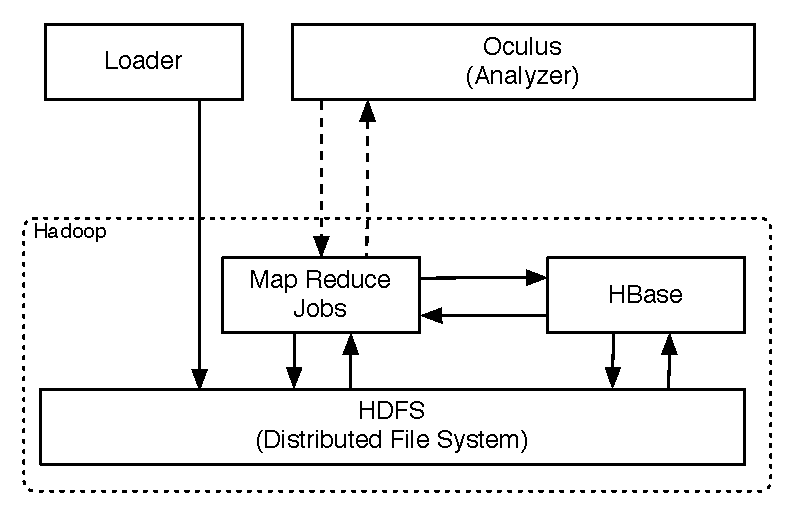
\includegraphics[scale=0.9]{./diagrams/high-level-system.pdf}
  \caption{High level overview of the system's architecture}
  \label{fig:system-overview}
\end{figure}

This section will focus on describing the general design of both systems, first the Loader's actor-based cluster model, and then the Analyser's Hadoop-backed batch processing cluster.

% ------------------------------------------------------------------------------------------------------------------------------------------------
\section{Loader}
\label{sec:loader-basics}
The Loader component is responsible for obtaining as much as possible ''reference data'', by which video material from sites such as \textit{youtube.com} or video hosting sites is meant. Please note that for the sake of this thesis (and legal safety) the downloaded content was limited to movie trailers (which are freely available on-line) as well as series opening or ending sequences.

While the Loader system will be referred to from here on in singular, it should be noted that in fact there are multiple instances of it running in the cluster. Thanks to the use of Akka's \textit{Cluster} module \cite{akka-cluster}, it was also fairly easy to distribute actors among multiple physical nodes in the cluster, allowing the actor system to utilise the entire cluster's processing power. The use od messaging as default and only mean of communication with actors allowed to easily transition into the clustered model, where communication would he handled over the network, from a previously local-only model.

\subsection{Types of Actors used in the system}
\label{sec:types-of-actors}

The system consists of 4 types of Actors. Each of them has multiple instances which are spread out on many nodes in the cluster. Some tasks can only be sent to local Actors (any work requiring an already downloaded file), but messages related to crawling and initially downloading the video material can be spread throughout the cluster. 

The following Actor descriptions are aimed at explaining the protocols used for comunication between them in the running system. These are very important as actors can communicate only via sending and receiving messages, and can not provide any type signatures that would help to identify what messages they can respond to. The also do not have methods that can be called directly on them -- this is a direct result of implementing actor model based concurrency, which would not be able to hold in face of direct access to an actors state.

will now briefly describe the different Actor roles that exist in the system and then explain the interactions between then on an example.

\begin{itemize}
  \item \textbf{YouTubeCrawlActor} -- is capable of fetching and YouTube websites and generate Messages triggering
                                    either further crawling of ''related video sites'' (\verb|Crawl(siteId: String)|) or downloading of the 
                                    currently accessed video (by sending a \verb|Download(movieId)| message),
    \subitem  \textbf{receives:}
      \subsubitem 1 -- \verb|Crawl(siteId: String)| message
    \subitem  \textbf{sends:}
      \subsubitem 0 or n -- \verb|Crawl(siteId: String)| - where n is the number of ''related video'' links found on the site. 
                                                           If crawling is turned off, no messages will be sent.

  \item \textbf{DownloadActor} -- is responsible for downloading the movie from youtube in it's original format (in the presence of many formats, 
                                the highest quality file will be downloaded). This Actor decides if a video is legal to download or not, because it also
                                obtains the movie's metadata -- only trailers and opening sequences of series are downloaded during for the sake of this 
                                thesis.
                                
  \item \textbf{ConversionActor} -- is responsible for converting the downloaded video material into raw frame data (bitmaps).
    \subitem  \textbf{receives:}
      \subsubitem \verb|Convert(localVideoFile: java.util.File)| -- This message must come from a local Actor, since the path refers to the local file system.
    \subitem  \textbf{sends:}
      \subsubitem \verb|Upload(framesDirectory: java.util.File)| -- when the finished converting to bitmaps, it will send and \verb|Upload| message to one of the\verb|HDFSUploadActors|, pointing to the directory where the output bitmaps have been written.
                                                                    
  \item \textbf{HDFSUploadActor} -- is responsible for optimally storing the sequence of bitmaps in Hadoop. This includes converting a series of 
                                  relatively small (around 2MB per frame) files into one Sequence File on HDFS. Sequence Files and the need for their use
                                  will be explained in detail in section \ref{sec:sequence-files}.
  \subitem \textbf{receives:}
    \subsubitem \verb|Upload(framesDirectory: java.util.File)| -- pointing to a local directory where the bitmap files have been stored.
                                                                 This message must come from a local actor, since the path refers to the local file system.
    \subitem  \textbf{sends:}
      \subsubitem 0 or 1 -- \verb|ConfirmUpload(localFile: java.util.File)| -- sent back to the sender that requested the video to be uploaded.
\end{itemize}

Using these Actors and protocols between them, the application is able to progress safely without the possibility of getting stuck in a dead (or live) lock. 

While discussing there protocols one should also mention that the messages that can be received and sent by Actors are not possible to verify using static typing -- an Actor can receive a message of ''Any'' type, and in case of not being able to act upon it - it will drop the message, but the delivery still happens.
This is an inherent property of the Actor Model of concurrency -- which is why in such systems explaining the flows of mesages and Actors present in the system is of such importance. Having this in mind, the next Section (\ref{sec:obtaining-reference-material}) will focus on explaining one such message flow within the system.

% -------------------------------------------------------------------------------------------------------------------------------------------------
\subsection{Obtaining reference video material}
\label{sec:obtaining-reference-material}
This section wills discuss the process of obtaining video material by the Loader subsystem, as well as explain which parts can be executed on different nodes of the cluster. The Figure \ref{fig:high-level-loader} should help in understanding the basic workflow.

\begin{figure}[ch!]
  \centering
  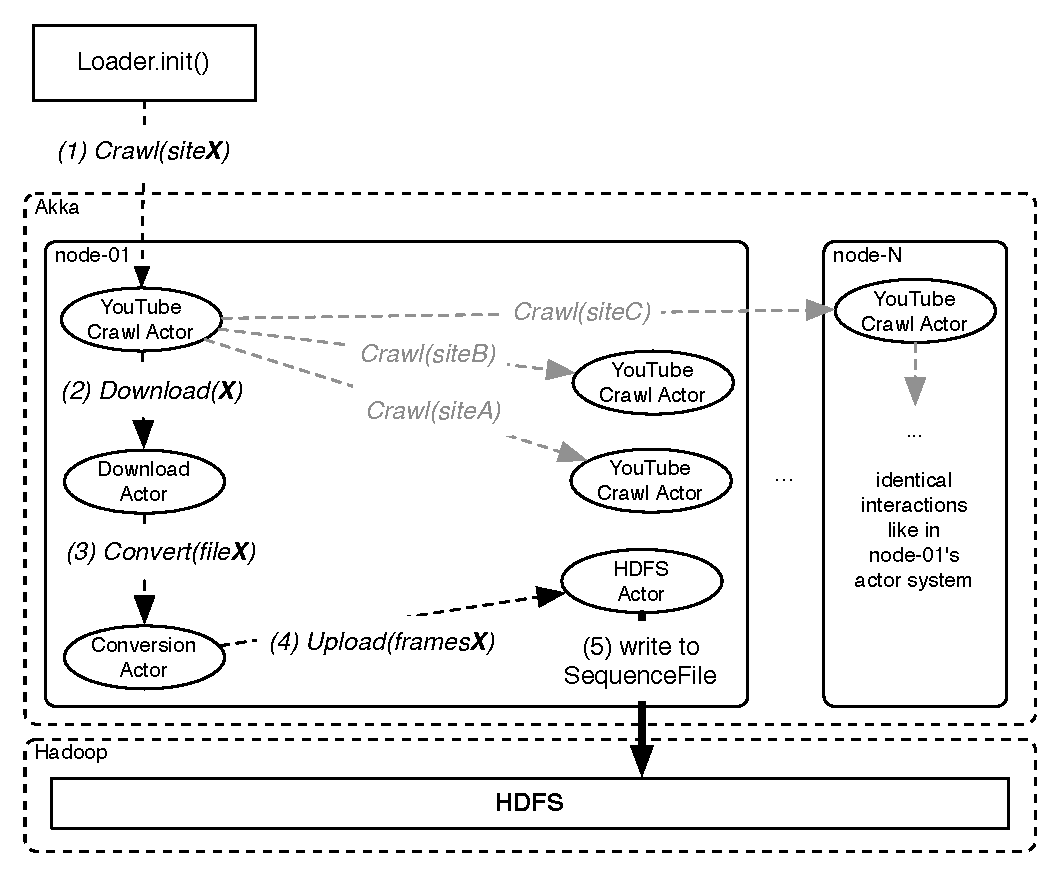
\includegraphics[scale=0.9]{./diagrams/loader-high-level.pdf}
  \caption{Overview of messages passed within the Loader's actor system. Greyed out messages are also sent, but are not on the critical path leading to obtaining material from \textit{siteX} into HDFS.}
  \label{fig:high-level-loader}
\end{figure}

\subsubsection{Step 1 - \textit{Crawl} messages}
The initiating message for each flow within the Loader is a \textit{Crawl(siteUrl)}, where siteUrl is a valid youtube video url.
The receiving YouTubeCrawlActor will react to such message by fetching and extracting the related video site urls and will forward those using the same kind of \textit{Crawl} messages. The second, yet most important, reaction is sending a \textit{Download(movieId)} message to an instance of an DownloadActor -- it  can reside on any node in the cluster, which allows us to spread the down-link utilisation between different nodes in the cluster.

It is worth pointing out that the receivers of these messages can be \textit{remote} Actors, that is, can be located on a different node in the Cluster than the sender. In order to guarantee spreading of the load among the many actors within the system (across nodes in the cluster), a routing strategy called ''Smallest Inbox Routing'' was used. This technique uses a special ''Router Actor'' which is responsible for a number of Routees (target Actors), and decides to deliver a message only to the Actor who has the smallest amount of messages ''not yet processed'' (which are kept in an Queue called the ''Inbox'', hence the strategy's name).

\subsubsection{Step 2 - \textit{Download} messages}
In the second step an \textit{YouTubeDownloadActor} instance receives a message asking it to download a movie.
It does so by invoking the native app \textit{youtube-dl}, which is an open source program specialised in downloading movies from YouTube.
Other than the video file (in an open source format) we also download a metadata description during this step, such metadata includes for example the date of publication, author, title and description of the movie. From this message including, all messages will be routed only to Actors local to the current node, because messages include \textit{File} objects, pointing to locations on-disk.

The metadata is then used to determine if it can be used in the context of this work, as only movie trailers and and opening / ending sequences are downloaded into the Oculus system. If the content is OK to use, the Actor sends an \textit{Convert(movieLocation)} message to an instance of \textit{ConversionActor}.

\subsubsection{Step 3 - \textit{Convert} messages}
The next step is executed by an instance of an \textit{ConversionActor} recieving an \textit{Convert(file)} message from another (local) Actor. The conversion phase will extract raw frame data from the incoming movie, and write those as plain bitmaps (not compressed) to files (one per each frame) into a specified target directory. The reason for not using a compressed lossless image format here is that all algorithms that the system will be dealing with later on are dealing with the raw image data, so we can avoid having to go over uncompression phases each time we will process a frame. Having that said, the storage format used for storing these files on HDFS provides build in compression (if enabeled), and it should be preferred in this case as it is transparent for the application, easing development of Map Reduce jobs in the Analyser system immensely.

The conversion from movie to raw bitmaps is performed by running an native application called \verb|ffmpeg| \cite{ffmpeg} instance (an de facto standard tool for such media operations), by forking a process from within the Actor. The CPU usage of running this extraction process easily reaches 100\% of the available resources, which is why the number of Conversion Actors per node is limited to only 1 per node, allowing ffmpeg to consume all available resources and finish extracting the data sooner. The actor will block until the process completes, and will then continue by sending an \textit{Upload(bitmapDirectory)} message to one of the \textit{HDFSUploadActors}.

\subsubsection{Step 4 \& 5 - \textit{Upload} messages}
The last step is an \textit{HDFSUploadActor} recieving an \textit{Upload(bitmapDirectory)} message which triggers it to connect to HDFS and start writing the bitmap data contained in the given directory to HDFS. The format of the generated data is as previously mentioned one file per frame of video, which averages around 2MB (depending on the movie resolution).

In this step the important part is that it does not write these files 1:1 onto HDFS, but instead writes into one file, using a hadoop specific storage format called ''Sequence File'', which allows for more efficient storage and latter retrieval of this data. Sequence Files, the need and benefits gained by using them as storage format for ''frame by frame'' data will be discussed in Section \ref{sec:sequence-files}.

This write terminates the operations performed on one movie by the Loader. All other operations will be performed by the Analyzer by running Map Reduce jobs on Sequence Files prepared in the above flow.

\subsection{Loader design summary}
As was explained in the previous sections the Loader is designed as fully asynchronous system, composed of Actors performing very specific tasks. All communication between the Actors is implemented as message passing, which provides so-called ''location transparency'' between the Actors -- this property has been utilised to spread the work-load between multiple nodes in a clustered enviroment, enabeling the work to be completed faster than only utilising a single node.

A detailed discussion of the Cluster's scalability and patterns applied in order to provide ad-hoc joining of nodes to the computation cluster can be found in Section \ref{chap:perf-scalability}: ''Scaling out the Ator system based Cluster''.

% ------------------------------------------------------------------------------------------------------------------------------------------------
\section{Analyser}
\label{sec:analyser}
The analyser component is responsible for orchestrating Map Reduce jobs and submitting them to the cluster. Results of jobs are written to either HBase or plain TSV (\textit{Tab Separated Values}) Files. Figure \ref{fig:analyser-high-level} depicts the typical execution flow of an analysis process issued by Oculus.

\begin{figure}[ch!]
  \centering
  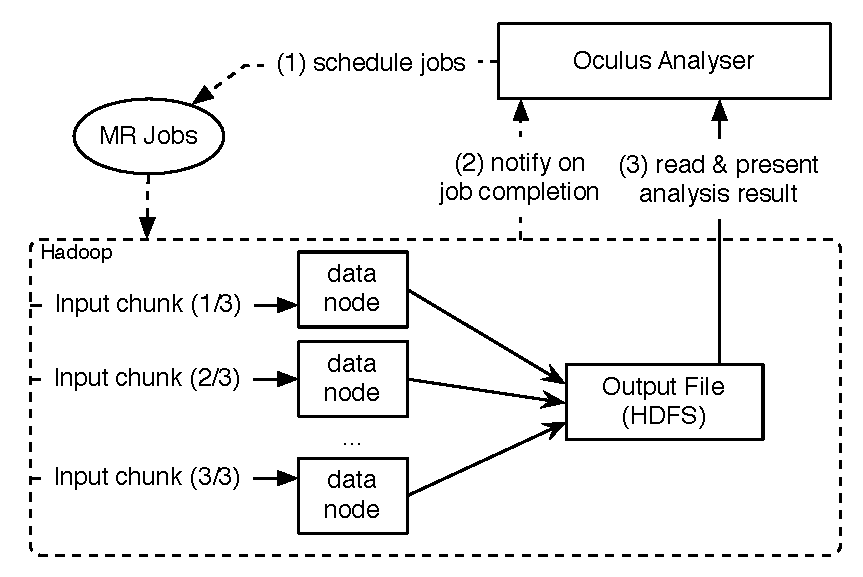
\includegraphics[scale=0.9]{diagrams/analyser-high-level.pdf}
  \caption{When storing a small file in HDFS, it still takes up an entire block. The grey space is not wasted on disk, but causes the \textit{name-node} memory problems.}
  \label{fig:analyser-high-level}
\end{figure}

In step 1 the \textit{job pipeline} is being prepared by the program by aggregating required metadata and preparing the job pipeline, which often consists of more than just one Map Reduce job -- in fact, most analysis jobs performed by Oculus require at least 3 or more Map Reduce jobs to be issued to the cluster. It is important to note that some of these jobs may be dependent on another task's output and this cannot be run in parallel. On the other hand, if a job requires calculating all histograms for all frames of a movie as well as calculating something different for each of these frames -- these jobs can be executed in parallel and will benefit from the large number of data nodes which can execute these jobs.

The 2nd step on Figure \ref{fig:analyser-high-level} is important because Oculus may react with launching another analysis job based on the notification that one pipeline has completed. This allows to keep different pipelines separate, and trigger them reactively when for example all it's dependencies have been computed in another pipeline.

For most applications though the 3rd step in a typical Oculus Job would be to read and present top N results to the issuer of the job, which for a question like ''Which movie is similar to this one?'' would be the top N most similar movies (their names, identifiers as well as match percentage).

The following sections (\ref{sec:deployment-strategy}, \label{sec:defining-pipelines-basics}) will introduce the cluster deployment as well as how Jobs are implemented on top of it, in order to parallelize the job's execution as much as possible.



% ------------------------------------------------------------------------------------------------------------------------------------------------
\subsection{Hadoop Cluster deployment strategy}
\label{sec:deployment-strategy}

Since the Analyser is most dependent on the Hadoop cluster's deployment this section aims to introduce the cluster's components and initial (3 node) setup. 

While this section only only introduces the various components of the cluster and it's initial deployment, chapter \ref{chap:perf-scalability} (''Cluster scaling and performance analysis'') revisits this topic and will focus on details such as cluster configuration options as well as influence of the number of participating nodes in the cluster on total computation times will be measured and tuned to increase the cluster's efficiency.

\subsubsection{Initial Hadoop cluster deployment}

The Hadoop deployment described in this subsection will focus on two elements of the Hadoop ecosystem - the Hadoop Distributed File system (HDFS) and the Hadoop Map Reduce Runtime.

The minimal hadoop deployment consistst of \textit{5 individual processes}, each with an assigned and very specific role in the clusters functioning. These processes can be classified as running along side the NameNode or DataNodes. This distincion should be clear after listing the names and features of these processes.

Firstly, the 3 processess associated with the ''master'' node, which is responsible for being the entry point for HDFS file requests as well as Job submissions:

\begin{itemize}
  \item \textbf{NameNode} (HDFS) -- is responsible for mapping logical file paths to their locations on DataNodes within 
                                    the cluster. This component was a Single Point of Failure (SPOF) on Hadoop clusters 
                                    until version 2.0 implemented the so called High Availability (HA) module, which 
                                    allows the cluster to run a second (not to be confused with \textit{secondary}) 
                                    NameNode in the cluster in the case the primary would fail. The HA module was not 
                                    used during this thesis, as it was not required to ensure the cluster's high 
                                    availability as the data could always be easily obtained again.
  \item \textbf{SecondaryNameNode} (HDFS) -- is responsible for a process called ''checkpointing'' of the NameNode's 
                                            fsimage and it's edit-log. It's name may be very misleading, as at no point
                                            in time is the SecondaryNameNode able to take the primary NameNode's place -- 
                                            this can be only achieved by using the High Availability modules. Use of the 
                                            SecondaryNameNode though allows the NameNode to fail and re-join a running 
                                            cluster -- without the SecondaryNameNode that failed NameNode would have lost 
                                            all of it's file system state and a full HDFS restart (including all 
                                            datanodes) whould be required.
  \item \textbf{JobTracker} (MapReduce) -- is responsible for tracking Map Reduce Jobs running in the cluster. It behaves 
                                           like a queue, in taking Job requests and processes them in order (or based on 
                                           customasible strategies). It is also in contact with all TaskTrackers 
                                           (described below), which actualy perform the work related to a MR Job, while 
                                           the JobTracker only gets and aggregates the job's progress. In case of failed 
                                           Jobs or Tasks it can also restart or redistribute the job to other DataNodes.
\end{itemize}

The distribution of these processes within the initial 3 node deployment is shown on Figure \ref{fig:small-cluster-deployment}.

\begin{figure}[ch!]
  \centering
  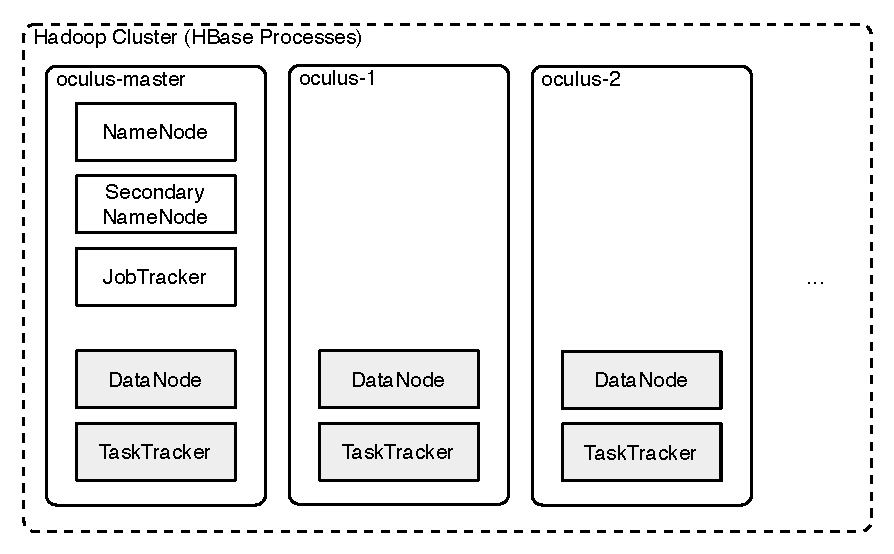
\includegraphics[width=0.8\textwidth]{img/hdfs-processes}
  \caption{Deployment diagram of the various HDFS processes within the initial 3-node cluster.}
  \label{fig:small-cluster-deployment}
\end{figure}


\subsubsection{HBase deployment}
\label{sec:hbase-deployment}
\todo{hbase deployment}s

\begin{figure}[ch!]
  \centering
  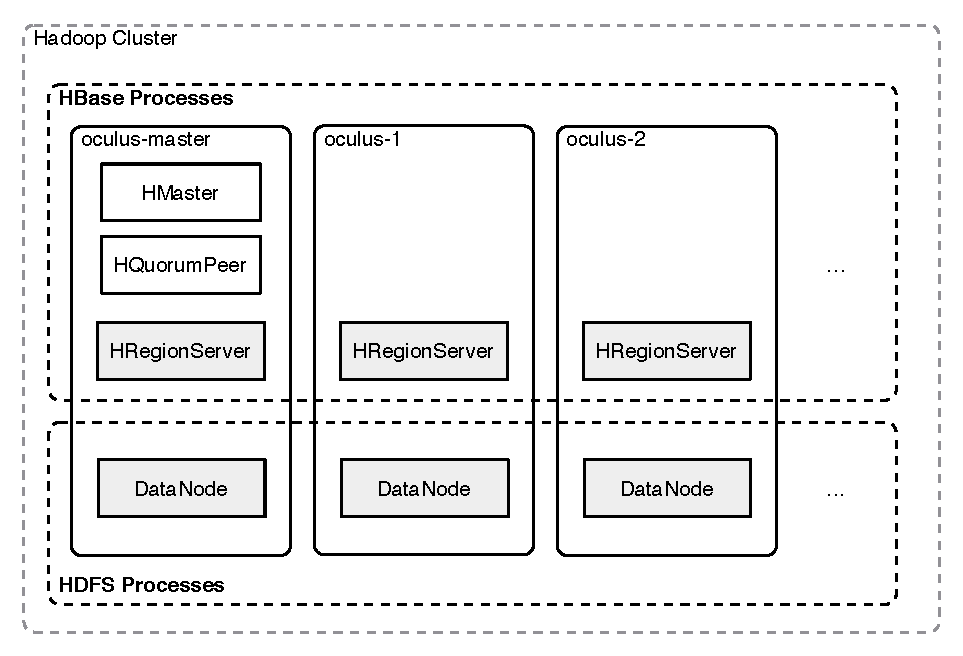
\includegraphics[width=0.8\textwidth]{img/hbase-processes}
  \caption{Deployment diagram of the various HDFS processes within the initial 3-node cluster.}
  \label{fig:small-cluster-deployment}
\end{figure}

Since HBase is so tightly connected with HDFS through direct use of it's DataNodes, all configuration changes connected to the HDFS cluster directly influence Hbase's behavior, for better or worse.


% ------------------------------------------------------------------------------------------------------------------------------------------------
\subsection{Defining Map Reduce Pipelines using Scalding and Cascading}
\label{sec:scalding-jobs}
The language and for implementing these processing pipelines used in this thesis was Scalding -- Twitter's home grown Scala DSL, which was already briefly introduced in Section Section \ref{sec:scalding-info}. The choice of using Scalding, and not Hadoop's plain Map Reduce API was mostly dictated by understandability and ease of modifying complicated job pipelines. 

\subsubsection{Comparison of example Job implemented using Plain Hadoop and Scalding}

This section aims to demonstrate what gains using Scalding over Hadoop yields, by showing the smallest possible example of an Map Reduce Job, implemented using both plain Hadoop APIs as well as Scalding. One should remember that Scalding is not a different framework than Hadoop, and in the end it will produce the exact same computations and classes (one instance of an \verb|Mapper| and one instance of an \verb|Reducer|).

The example shown on the below listings is a Hadoop equivalent of what programming languages aim to demonstrate using ''Hello World!'' applications -- it is a minimal piece of code showing the working of the given technology. The task to solve is defined as: ''\textit{Given a huge input text file, count the occurances of each discrete word, and return a summary of these}''. As the aim of Hadoop is to leverage parallel computing, the classic method of implementing this task is to emit tuples of \verb|(word, 1)| for each word, then relying on Hadoops internal mechanisms to group such tuples together by the first value (the \verb|word|), and reducing these into a tuple of \verb|(word, sum(1,1,1,...))| during the Reduce step.

The difference in complexity should be obvious by comparing the Listing \ref{lst:hadoop-mr} which represents the Map and Reduce classes which are used to represent the respectful Map and Reduce functions in the Java API, with Listing \ref{lst:scalding-wc} which is the complete code for a job performing the exact same in Scalding's Scala Domain Specific Language. 

\begin{lstlisting}[caption={Word Count example Job, implemented using plain Java Map Reduce API}, label={lst:hadoop-mr}]
public class Map 
    extends MapReduceBase 
    implements Mapper<LongWritable, Text, Text, IntWritable> {

 private final static IntWritable one = new IntWritable(1);
  private Text word = new Text();

  public void map(LongWritable key, 
                  Text value, OutputCollector<Text, IntWritable> output, 
                  Reporter reporter) throws IOException {
   String line = value.toString();
   StringTokenizer tokenizer = new StringTokenizer(line);
   while (tokenizer.hasMoreTokens()) {
    word.set(tokenizer.nextToken());
    output.collect(word, one);
   }
  }
}

public class Reduce 
    extends MapReduceBase 
    implements Reducer<Text, IntWritable, Text, IntWritable> {

 public void reduce(Text key, 
                    Iterator<IntWritable> values, 
                    OutputCollector<Text, IntWritable> output, 
                    Reporter reporter) throws IOException {
  int sum = 0;
  while (values.hasNext()) sum += values.next().get();
  output.collect(key, new IntWritable(sum));
 }
}
\end{lstlisting}


\begin{lstlisting}[caption={Simplest Scalding job used in Oculus -- each frame perceptual hashing}, label={lst:simplest-scalding-job}]
  Tsv("input.tsv")
    .map('line -> 'word) { line: String => line.split }
    .groupBy('word) { _.count }
    .write(Tsv("output.tsv"))
\end{lstlisting}

As seen on the previous listings, Scalding provides much more concise code, and thanks to this enables developers to focus on the algorithm, and not the boilerplace accompanying these kinds of applications.

\subsubsection{Defining advanced Job Pipelines using Scalding}
\label{sec:defining-pipelines-basics}
Scalding also provides powerful facilities for pipeline building, where by ''Pipeline'' we refer to a series of Jobs that use the output of a previous Job as the input for the next one. It is worth mentioning that this is not something plain Hadoop APIs are able to provide easily, and one would have to implement logic in Jobs that would store the intermediate output in a directory and await the Job's completion, to then manually start the second job (by running it's main method).

Building Pipelines has two major styles in Scalding: explicit ''next Job'' definitions, as well as implicit dependencies on results of Jobs. We will investigate both styles in this section -- starting with the explicit style, as it is more similar to the manual style of doing things.

\begin{lstlisting}[caption={Explicit ''next job'' definition within a Scalding Job class}, label={lst:next-job}]
case class FirstJob(args: Args) extends Job(args) {
  val in = args("in")
  val out = in + ".out"
  
  Tsv(in).read.write(Tsv(out))
  
  def next = Some(SecondJob(Args("--in", out)))
}

case class SecondJob(args: Args) extends Job(Args(out)) { /*...*/ }
\end{lstlisting}

Listing \ref{lst:next-job} shows how one can use Scalding to combine two Jobs using Scalding's DSL. The \verb|SecondJob| depends on the output of the \verb|FirstJob| (which in this case only copies the input to another file on HDFS), since the \verb|next| method is defined within the first Job, we have it's parameters available and can construct the next Job in the pipeline, providing it with it's required \verb|in| parameter. 

\begin{figure}[ch!]
  \centering
  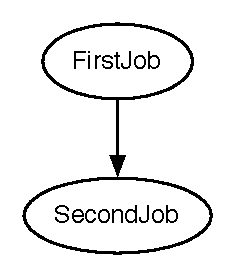
\includegraphics[width=0.25\textwidth]{img/simplest-pipeline}
  \caption{Simplest Job Pipeline, with SecondJob depending on the output of FirstJob (each circle being one Map Reduce Job).}
  \label{fig:simplect-pipeline}
\end{figure}

Such pipeline can be visualised as seen on Figure \ref{fig:simplect-pipeline}, which is an output generated by using the graphviz tool (as in "graph visualization"), applied to a file describing the graph as described in the DOT format. The DOT file corresponding to the graph depicted on Figure \ref{fig:simplest-pipeline} is shown in Listing \ref{lst:simplest-pipeline-dot}. DOT descriptions of pipelines are in common use among profesionals designing such systems, and can also be generated automatically by Scalding -- which is tremendously useful when working with very long pipelines.

\begin{lstlisting}[caption={Textual description of graph on Figure \ref{fig:simplect-pipeline}, using the DOT graph description language.}, label={lst:simplest-pipeline-dot}]
digraph G {
  1 [label = "FirstJob"];
  2 [label = "SecondJob"];
  
  1->2
}
\end{lstlisting}

The second way of building up pipelines is inside one Scalding Job file. Because Scalding's rich set of operations, what may look as simple on the surface (in the pipeline definition) may have to boil down to multiple Map Reduce Job executions. One obvious case that will cause one Scalding Job to produce multiple Map Reduce Jobs is using data from two separate sources and joining them together. It should be noticed that the notion of ''join'' (as known from relational databases) is something both very powerful and very foreign to Hadoop -- as it is only designed to deal with data in a batch-processing fashion. Scalding allows to express join operations trivially in the the definition file, but it's execution actually is quite complicated and forces all the data from one side of the join to be loaded into Mappers participating in the Job's execution.

\begin{lstlisting}[caption={Scalding job, reading data from 2 sources and joining them on dominantColor, producing 3 Map Reduce Jobs}, label={lst:read-and-join-scalding}]
class CompareByDominantColor(args: Args) extends Job(args) {
  // newly analysed video
  val analysedMovieFrames = 
    WritableSequenceFile(input, ("key", "value"))
    .read
    .rename("key", "frame")
    .map(("frame", "value") -> ("dominating", "red", "green", "blue")) { 
        p: (Int, BytesWritable) => calculateHistograms(p._2)
    }
  
  // reference database
  val referenceFrames = 
    HistogramsTable.read
    .rename("dominating", "refDominating")

  // join
  referenceFrames.joinWithSmaller(analysedMovieFrames, 
                                            "dominating" -> "refDominating")
    // operations on joined dataset
}
\end{lstlisting}

Listing \ref{lst:read-and-join-scalding} showcases a simple join operation, which is the core of the algorithms implemented in this thesis. This pipeline definition compiles down into 3 Map Reduce Jobs, because it reads from 2 separate data sources: from a sequence file that we just started processing (this is the movie this job aims to compare to the referece data set), and from the \verb|HistogramsTable| which is the reference dataset containing refernece data calculated previously for all already processed movies in the reference database. The \verb|HistogramsTable| refers to an \textit{HBase Table}, and during the Job's executionw will trigger (in this case) a full-scan over the entire ''histograms'' table stored in HBase - in practice it was feasible to sample down the sample count obtained from HBase, by applying the \verb|.sample(75.0)| operation to the larger data set. Figure \ref{fig:3-pipeline} shows the dependencies as modeled by this definition.

\begin{figure}[ch!]
  \centering
  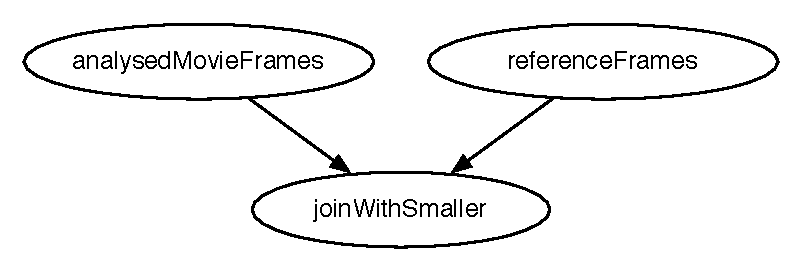
\includegraphics[width=0.75\textwidth]{img/second-simplest-pipeline}
  \caption{Join operation, forcing the Pipeline to consist of 3 Map Reduce Jobs (depicted as circles)}
\end{figure}


The dependencies, as seen on Figure \ref{fig:3-pipeline} between the first two Jobs to the 3rd ''Join Job'' were not explicitly modeled as previously seen using the \verb|next| method, and instead were inferred from the use of the \verb|job1.joinWithSmaller(job2, "key1" -> "key2"| operation. This is very important and useful because of two reasons:

\begin{itemize}
  \item Cascading is able to determine dependencies between Map Reduce jobs, and execute them on the Hadoop cluster as dictated by their dependency graph.
  \item Jobs that do not depend on each other's outputs can be run in parallel.
\end{itemize}

Thanks to the second property of these Job Pipelines (parallel execution of independent sub-graphs) total execution time of such Map Reduce Pipelines may be further optimised when running on large clusters.






% ------------------------------------------------------------------------------------------------------------------------------------------------
\chapter{Practical examples of distributed media analysis}
\label{chap:analysis-examples}

This chapter aims to provide tangible examples of how the previously described system preformed and what kind of information was extracted from the reference database when trying to match against disorted media inputs.

The following two sections will focus on practical examples of potential ''attacks'' (disortions) applied to the input media data, and how the proposed system has handled it. The examples have been selected to highlight the two major problems the system has to handle -- distorted image data and time shifted data.

In Section \ref{sec:mirrored-video-detection} video material will be analysed in order to find it's corresponding ''mirrored'' counter-part. This example will also be used to highlight the tremendous possibilities that lie within data \textit{pre-processing} that are applied within the proposed system, and if needed could be expanded even more in order to speed up the system's initial response time.

In Section \ref{sec:scene-detection} an extracted scene will be positioned within an existing video in the reference database. This problem turns out to be non-trivial because of different frame-rates of supplied material, thus search methods similar, in concept, to sub-string search could not have been applied efficiently. The section explains the algorithms applied instead, and showcases an example case.

As this thesis is not focused on development of image analysis algorithms, these sections will instead lean their focus towards the distributed system and big-data parts of the problem. The image comparision algorithms also assume that that the used image correlation algorithm (\textit{phash} -- see Section \ref{sec:phash}) performs well enough for the job at hand. 

\textit{The frames used to illustrate the experiments originate from the movie ''\textit{Big Buck Bunny}'' \cite{big-buck-bunny} which has been created by the Blender Foundation \cite{blender-foundation} and released under the Creative Commons license \cite{creative-commons}.}

% ------------------------------------------------------------------------------------------------------------------------------------------------
\section{Mirrored video detection}
\label{sec:mirrored-video-detection}
In order to test the system in scenarios of image disortion the example case of ''mirrored'' video material was used. This case is fairly popular among material uploaded to YouTube, so outside of the ease of preparing test data, it is also a valid real-life scenario of one might encounter.

\begin{figure}
        \centering
        \begin{subfigure}[b]{0.45\textwidth}
                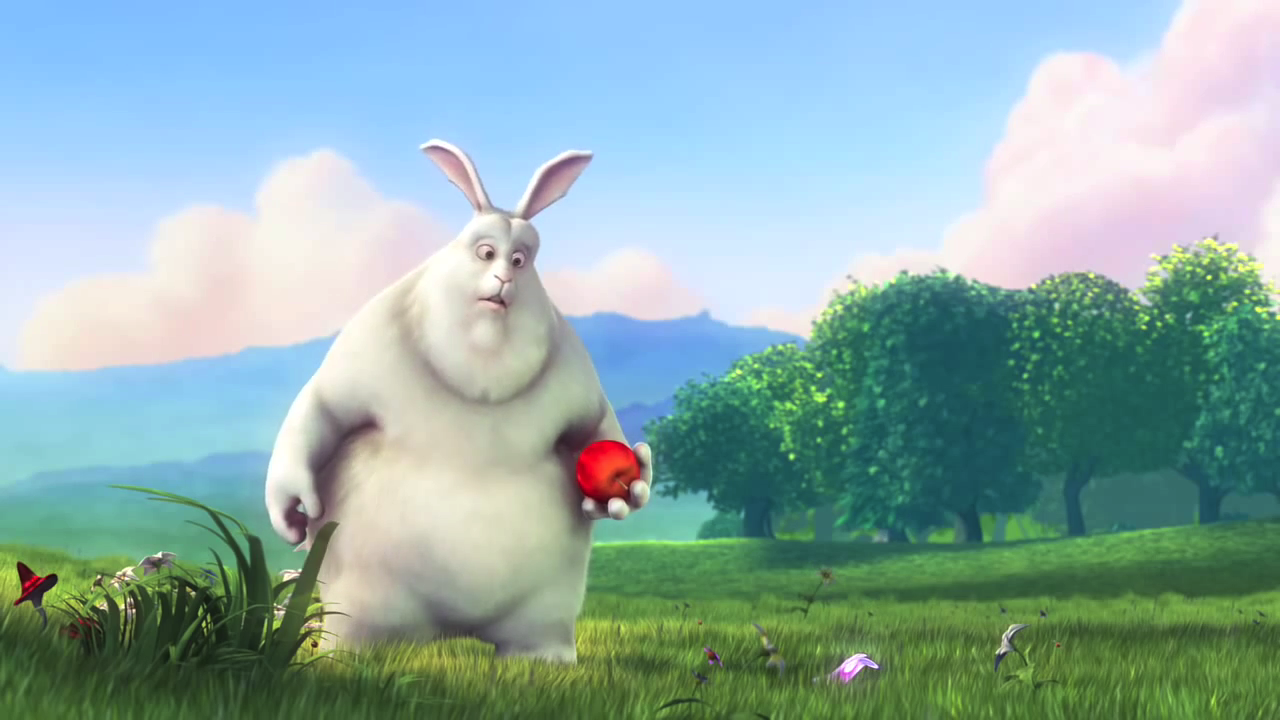
\includegraphics[width=\textwidth]{img/Big_Buck_Bunny_normal.png}
                \caption{Original frame}
                \label{fig:original-frame}
        \end{subfigure}
        \begin{subfigure}[b]{0.45\textwidth}
                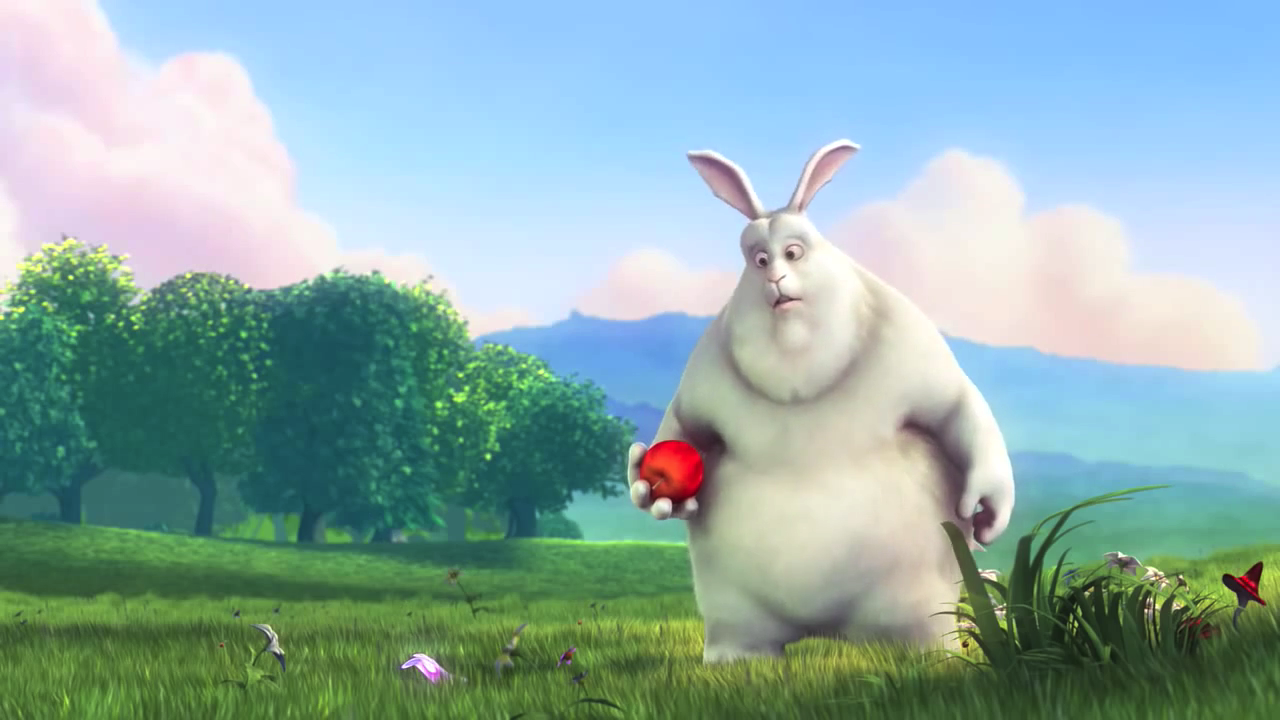
\includegraphics[width=\textwidth]{img/Big_Buck_Bunny_mirror.png}
                \caption{Mirrored frame}
                \label{fig:mirrored-frame}
        \end{subfigure}
        \caption{Example of original and mirrored frame}\label{fig:frames-mirrored}
\end{figure}


\subsection{Detecting other kinds of distorions in video material}

Of course, other kinds of disortions could be applied to a video, such as comparing a high-quality video with a low-quality counterpart or simple coloring filters. While being outside of the scope of this thesis, the basic concepts and framework proposed would easily be able to incorporate more scoring functions into the Map Reduce pipeline that would help determine matches between even such disorted video materials. 

An interesting example disortion found commonly in many materials is slight changes in the color hue or white balance of the \todo{histograms}


% ------------------------------------------------------------------------------------------------------------------------------------------------
\section{Scene detection}
\label{sec:scene-detection}
This scenario can be explained as trying to find out \textit{where} (if at all) a scene takes place in a movie known to the reference database. 

Although on the sufrace the general problem statement is not so different than substring search, which is a known and well researched topic in computer science. In sub-string search algorithms like the Knuth–Morris–Pratt \cite{kmp-string-search} or the Boyer-Moore \cite{boyer-string-search} algorithms leverage that the ''matching'' either will apply, or will not in order to increase search speed in the worst case to still linear time. However, these methods can \textit{not} be directly applied to the problem specified in this section -- because of the dissortions in source and reference video material as well as the possibility of cross-matches when a movie is built up from multiple short scenes from other movies -- a typical example here would be ''flash-back'' scenes or ''top 10'' movies where before the last top-3, the movie would quickly go over already shown frames of scenes. Another problem adding to the dissortions is frame rates of reference data vs. an analysed video fragment -- even a slight missmatch (30FPS vs. 25FPS) would render the substring search algorithms not usable for this concrete example.

\begin{figure}[ch!]
  \centering
  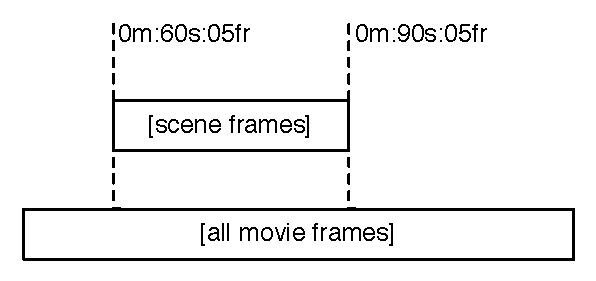
\includegraphics[width=0.6\textwidth]{img/frames-timeline-matching}
  \caption{Visual representation of the goal of this example application.}
\end{figure}

Instead, a more statistical aproach was taken. In which a frame is compared with it's set of ''potential match candidates'' which are determined by very coarse filtering of the reference data set by bucketing certain criteria of their histograms such as ''dominating red'' or ''dominating blue'' (this classification is prepared on the reference data beforehand -- during importing into the system).

\todo{mention somewhere before that we really extract data like ''mostly red''}

\todo{finish this scenario}

\begin{figure}[ch!]
  \centering
  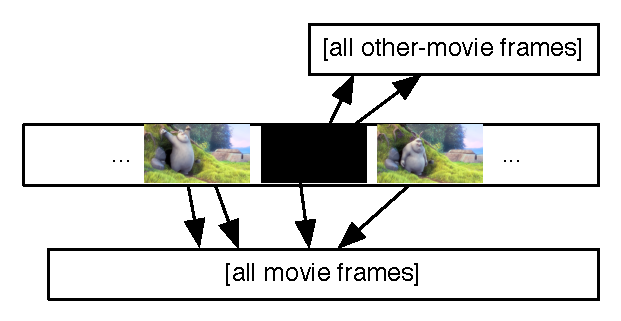
\includegraphics[width=0.6\textwidth]{img/frames-timeline-matching-missmatch}
  \caption{One frame may potentially match multiple reference frames. The final most probable matching scene is determined by aggregating data the direct frame-to-frame matches.}
\end{figure}

% --------------------------------------------------------------------------------

\section{Avoiding costy Map Reduce operations by limiting input sets}
\todo{explain that we use a subset of keys}



















% ------------------------------------------------------------------------------------------------------------------------------------------------
\chapter{Cluster scaling and performance analysis}
\label{chap:perf-scalability}

This section will focus on analysing as well as presenting improvements to the cluster deployment which can and have been applied to the Hadoop cluster leveraged by the Analyser application presented in previous chapters.

Section \ref{sec:scaling-hadoop} describes the multitude of challanges and problems encountered while scaling Hadoop cluster. It also describes three of the applied scaling and optimisation methods in detail -- including configuration changes as well as adding more nodes to the cluster.

% Section \ref{sec:optimising-hbase} discusses HBase specific optimisations that can be performed during application and data representation design. While all optimisations described in the previous section, which touch Hadoop's infrastructure also directly impact HBase performance, some very specific topics -- such as utilising HBase's guarantees about it's globally sorted row key and guaranteed random access times to specific row-keys make this topic worthy if it's own section.

Section \ref{sec:scaling-akka} will briefly explain scalability concerns related to an Akka based cluster deployment, yet as this component has not been as critical to overal system performance as the Analyser and Hadoop cluster, the Akka cluster has been deemed ''good enough'' for the scope of this paper.

Lastly Section \ref{sec:scaling-summary} will summarise the findings from the scaling experiments conducted in the previous sections, by stating general recommendations and hints for scaling systems that process larget amounts of data.

% ------------------------------------------------------------------------------------------------------------------------------------------------
\section{Scaling the Analyser's Hadoop Cluster}
\label{sec:scaling-hadoop}
This section will focus on analysing and tuning the various settings of the Hadoop cluster deployed for the previously described Analyser application. Subsections focus on tuning the cluster on a setting--by--setting basis yet the tuning will always be enforced by a business need, which in this case will be represented as the need to speed up processing of the map reduce pipelines producing results which were explained in Chapter \ref{chap:analysis-examples}.

\subsection{Storing images on HDFS, while avoiding the ''Small Files Problem''}
\label{sec:sequence-files}
Most algorithms used in Oculus operate on a frame-by-frame basis, which means that it is most natural to store all data as ''data for frame 343 from movie XYZ''. This applies to everything from plain bitmap data of a frame to metrics such as histograms of colours of a given frame or other metadata like the extracted text content found in this frame.

Sadly this abstraction does \textit{not} work nicely with Hadoop, it would cause the well--known ''small-files problem'' which leads to \textit{major} performance degradation of the Hadoop cluster is left unadressed. This section will focus on explaining the problem and what steps have been taken to prevent it from manifesting in the presence of millions of ''frame-by-frame'' pieces of data.

Hadoop uses so called ''blocks'' as smallest atomic unit that can be used to move data between the cluster.
The default block size is set to \textit{64 megabytes} on most Hadoop distributions.

This also means that if the DFS takes a write of one file (assuming the \textit{replication factor} equals 1) it will use up one block. By itself this is not worrying, because other than in traditional (local) file systems such as EXT3 for example, when we store N bytes in a block on HDFS,
the the file system can still use block's unused space. Figure \ref{fig:no-sequence-file} shows the structure of a block storing only one frame of a movie.

\begin{figure}[ch!]
  \centering
  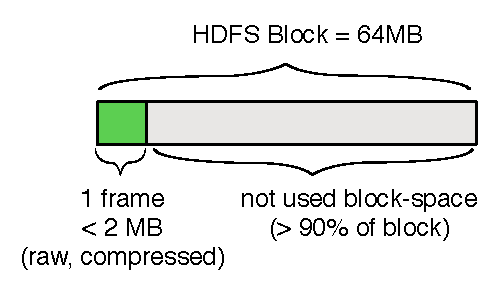
\includegraphics[scale=0.9]{diagrams/no-sequence-file.pdf}
  \caption{When storing a small file in HDFS, it still takes up an entire block. The grey space is not wasted on disk, but causes \textit{name-node} to store 1 block entry in memory.}
  \label{fig:no-sequence-file}
\end{figure}

The problem stemming from writing small files manifests not directly by impacting the used disk space, but in increasing memory usage in the clusters so called \textit{name-node}. The name-node is responsible for acting as a lookup table for locating the blocks in the cluster. Since name-node has to keep 150KB of metadata for each block in the cluster, creating more blocks than we actually need quickly forces the name-node to use so much memory, that it may run into long garbage collection pauses, degrading the entire cluster's performance. To put precise numbers to this -- if we would be able to store 500MB of data in an optimal way, storing them on HDFS would use 8 blocks -- causing the name node to use approximately 1KB of metadata. On the other hand, storing this data in chunks of 2MB (for example by storing each frame of a movie, uncompressed) would use up 250 HDFS blocks, which results in additional 36KB of memory used on the name-node, which is 4.5 times as much (28KB more) as with optimally storing the data! Since we are talking about hundreds of thousands of files, such waste causes a tremendous unneeded load on the name-node.

It should be also noted, that when running map-reduce jobs, Hadoop will by default start one map task for each block it's processing in the given Job. Spinning up a task is an expensive process, so this too is a cause for performance degradation, since having small files causes more \textit{Map tasks} being issued for the same amount of actual data Hadoop will spend more time waiting for tasks to finish starting and collecting data from them than it would have to.

% ------------------------------------------------------------------------------------------------------------------------------------------------
\subsubsection{Sequence Files}
\label{sequence-file}
The solution applied in the implemented system to resolve the small files problem is based on a technique called ''Sequence Files'', which are a manually controlled layer of abstraction on top of HDFS blocks. There are multiple Sequence file formats accepted by the common utilities that Hadoop provides \cite{hadoop-seq-files} but they all are \textit{binary header-prefixed key-value formats}, as visualised Figure \ref{fig:sequence-file}.


\begin{figure}[ch!]
  \centering
  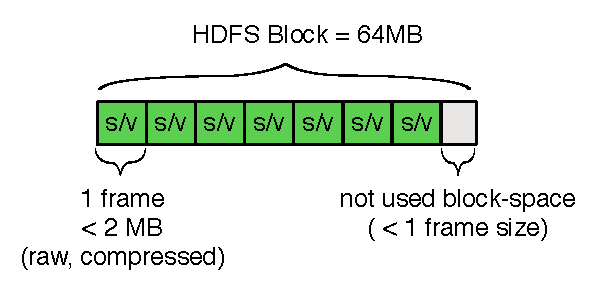
\includegraphics[scale=0.9]{diagrams/sequence-file.pdf}
  \caption{A SequenceFile allows storing of multiple small chunks of data in one HDFS Block.}
  \label{fig:sequence-file}
\end{figure}

Using Sequence Files resolves all previously described problems related to small files on top of HDFS. Files are no longer ''small'', at least in Hadoop's perception,
since access of frames of a movie is most often bound to access other frames of this movie we don't suffer any drawbacks from such storage format.

Another solution that could have been applied here is the use of HBase and it's key-value design instead of the explicit use of Sequence Files, yet this would not yield much performance nor storage benefits as HBase stores it's Table data in a very similar format as Sequence Files. The one benefit from using HBase in order to avoid the small files problem would have been random access to any frame, not to ''frames of this movie'', but since I don't have such access patterns and it would complicate the design of the system I decided to use Sequence Files instead.



% ------------------------------------------------------------------------------------------------------------------------------------------------
\subsection{Tuning replication factors, for increased job computation speed}
\label{sec:tuning-replication-factors}
One of the many tuneable aspects of Hadoop deployments that can have a very high impact on the clusters performance is the \textit{replication factor}, which stands for ''the number of datanodes a piece of data is replicated to''. This section will explain in detail how a tuning this factor, and leveraging Hadoop's scheduling mechanisms can be tweaked to trade of storage space (higher replication factors) to faster execution times of jobs.

Hadoop's primary strength in big data applications lies within leveraging \textit{data locallity} whenever possible. The concept of data locallity means that instead of moving the data around in the cluster, to a node where the application is running, the Task Scheduler will try find such ''map slots'' (multiple such slots can be assigned to one data node) that the data the job needs to process will be local to the node the slot resides on. Effectively this means that application code (jar and class files) will be sent to the executing server, and not the inverse. The rationale behind this measure is that the amounts of data are way bigger than the size of applications in these kinds of systems -- thus, avoiding to move the data can save both costs and precious time.


\begin{figure}[ch!]
  \centering
  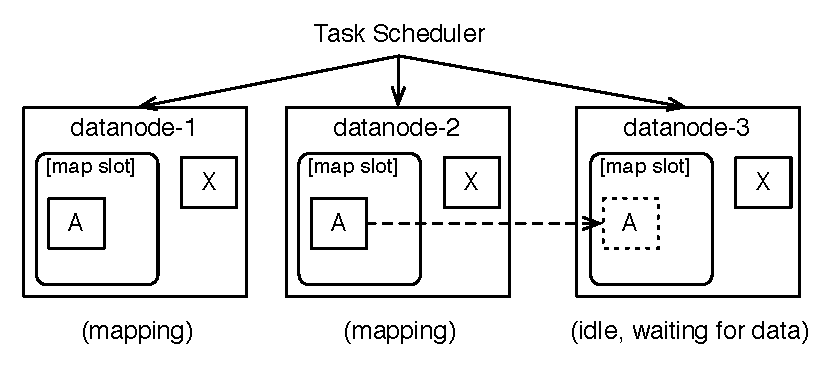
\includegraphics[width=\textwidth]{img/forced-data-replication.pdf}
  \label{fig:replication-ad-hoc}
  \caption{Three node cluster, with idle 3rd node; Scheduler will replicate data A while running the Job, in order to start a task requireing A on the 3rd idle node.}
\end{figure}


While data locallity is a \textit{priority} for the scheduler, it is by no means a hard requirement. In a scenario outlined in Figure \ref{fig:replication-ad-hoc} a job has been submitted to a 3-node cluster. The replication factor in the cluster is set to 2 -- which can be noticed by the number of times each piece of data is replicated among the datanodes. In the absence of any other jobs scheduled on the cluster, the fair--scheduler will decide to use the 3rd data node in order to accelerate the processing of the job, even though it does not have the required piece of data located on it (splits of A). Replicating the data over to datanode-3 is quite costly, and even though it may speed-up the total compute time, we loose time on transfering the data in an ad-hoc fashion.

By tweaking the replication factor for the given file, which we expect to be needed on more nodes, we can speed up the total compute time of a given job. In order to change the replication factor of a given path, one can use either the Java APIs or the hadoop command line tool, as shown in Listing \ref{lst:cli-change-replication}.

\begin{lstlisting}[caption={Explicitly changing the replication factor on a path using command line tools}, label={lst:cli-change-replication}]
hadoop dfs -setrep -R -w 3 /oculus/source/e98uKex3hSw.mp4.seq
\end{lstlisting}

By increasing the replication factor of paths that we know they will be used in many mappers, we can increase the number of data-local slots available to the scheduler, and avoid having to migrate the data in an ad-hoc fashion. Of course, the tradeoff is requireing even more disk space in the cluster, but it is well worth considering to raise the replication factor of a path while it is ''hot'', and lowering it afterwards.

\begin{figure}
  \centering
  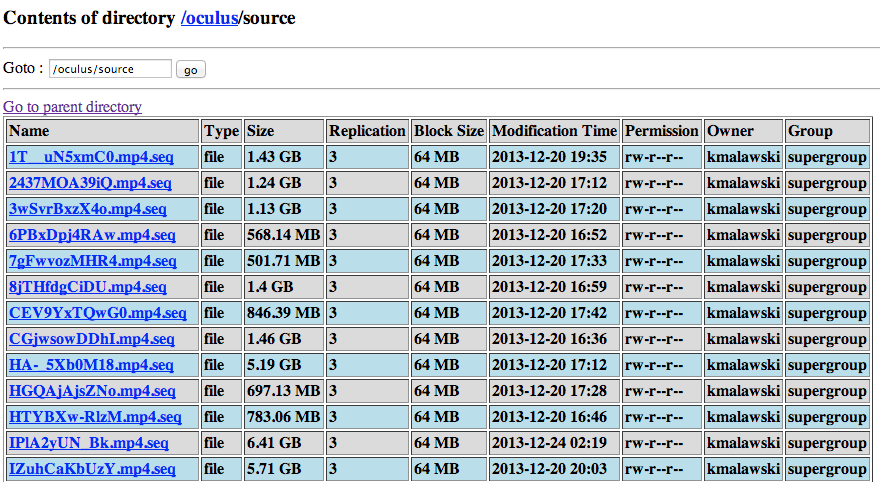
\includegraphics[width=\textwidth]{img/hadoop/hdfs_show-replication}
  \label{fig:hdfs-replication-factors}
  \caption{HDFS on-line browser, running on datanode (port: 50075), displaying replication factors of files (4th column)}
\end{figure}

The replication factor of a file (or path) is such an important value, it's usually always displayed along side any file listing within the Hadoop UIs (see Figure \ref{fig:hdfs-replication-factors}) as well as command line tools. It should also be noted that it is impossible to set the replication factor to a higher number than there are datanodes present in the cluster -- as the replication requirement would not be possible to be fulfilled.


\subsection{Tuning the Cluster's size, in conjunction with replication factors}
\label{sec:tuning-number-of-nodes}
Hadoop aims to deliver on the promise of ''nearly linear horizontal scalability'', which means that speed-up expirienced from adding more nodes to the cluster should impact the processing times positively in a linear fashion. Of course, adding more nodes also means that operational costs are higher, so one has to ballance the number of nodes with their fine-tuning as well as project needs. In order to test the systems behavior, the cluster was configured with 1 map slot on each datanode, and was initially running using 3 datanodes. This section aims to verify the horizontal scalability of the produced cluster, in the case of CPU intensive tasks -- such as computing phashes and histograms from movies (the pre-processing step as explained in Chapter \ref{chap:analysis-examples}.

Because the Map Reduce framework relies on parallelising computing of the map function supplied by the user, the goal of the cluster administrator should be to enable the maximum number of map slots. A map slot is defined as one ''slot'' in which the task scheduler may allocate work, in order to process a part of the map computation. The same can be specified for the reduce step, in which case one refers to \textit{reduce slots}.

\subsubsection{Growing the cluster}
\label{sec:growing-the-cluster}
With the base size of the cluster being 3 nodes (with one virtual machine hosting the namenode as well as a datanode, and the rest hosting only datanodes), this section aims to determine the horizontal scalability of the cluster, by sheer adding of datanodes to the hadoop cluster.

Adding nodes to the cluster is a very simple operation, and can be performed without any disruption of the already running cluster. During the tests performed for this section, additional VMs have been provisioned and added to the cluster by using the commands shown in Listing \ref{lst:adding-new-node-cluster}. It should be noted that the provisioned VMs would re-use an existing snapshot image of an instance prepared using OpsCode Chef, which is an configuration provisioning tool explained in detail in Appendix \ref{app:chef}. 

\textbf{The average time from starting a new node on Google Compute Engine, and it joining the Hadoop cluster is \textit{less than 1 minute} -- including the time to provision the fresh virtual machine!}

\newpage
\begin{lstlisting}[caption={Complete listing of adding a new worker node to the cluster, using GCE}, label={lst:adding-new-node-cluster}]
// provision new instance
gcutil --service_version="v1" --project="oculus-hadoop" adddisk "oculus-4b" --zone="us-central1-a" --source_snapshot="oculus-slave-snapshot"

gcutil --service_version="v1" --project="oculus-hadoop" addinstance "oculus-4b" --zone="us-central1-a" --machine_type="n1-standard-1" --network="default" --external_ip_address="ephemeral" --service_account_scopes="https://www.googleapis.com/auth/..." --tags="hadoop,datanode,hbase" --disk="oculus-4b,deviceName=oculus-4b,mode=READ_WRITE,boot" --auto_delete_boot_disk="true"

// obtain ip address
gcutil getinstance oculus-3b | grep ip
// ip               10.240.80.181
// external-ip  146.148.47.191

// add internal ip to namenode masters config
gcutil ssh oculus-master
echo "10.240.80.181" >> /opt/hadoop.1.2.1/conf/slaves

// start workers on added nodes
/opt/hadoop-1.2.2/start-all.sh

// add node aliases to local hosts
echo "146.148.47.191  oculus-3b" >> /etc/hosts
\end{lstlisting}

The job used to measure the impact of adding new nodes was the most CPU intensive task present in the Oculus workflow, which is: computing the perceptual hash of each frame of a given movie. The movie selected for the process was the previously introduced ''Big Buck Bunny'' movie, amounting a total of 6.38 GB of frame data to process, split among 103 HDFS Blocks (each roughly 64 MB in size). Thanks to this large number of blocks, the task scheduler should be able to efficiently distribute the work to even large numbers of worker nodes. In fact, as visible on Figure \ref{fig:ten-mappers} with 10 mappers (10 datanodes, with 1 map slot each) are executing tasks from the same job in parallel, causing an obvious speedup in Map comptation.


\begin{figure}[ch!]
  \centering
  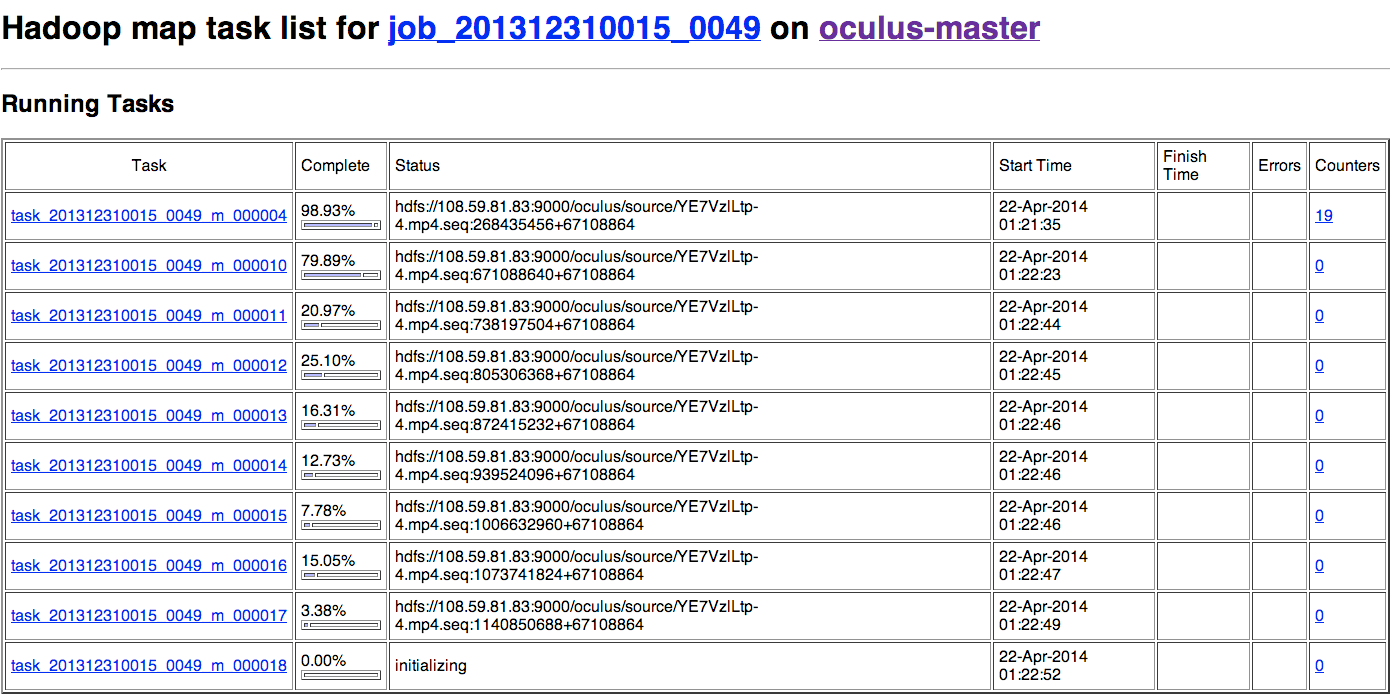
\includegraphics[width=\textwidth]{img/hadoop/10tasks-parallel}
  \label{fig:ten-mappers}
  \caption{Fragment of Web-UI interface displaying the progress of map tasks in the cluster consisting of 10 physical nodes, with one map slot each.}
\end{figure}

Before explaining the results of the performed scalability tests, one more term needs to be introduced. Tasks can be executed in a number of different ways -- that is, they may be executed strictly local to the data they work on, or just ''near the data the task requires'' or really ''far away from the data the task requires'' -- these intuitive definitions have their named counterparts which are measured and reported for every run of a Map Reduce job, namely those types of Tasks are:

\begin{itemize}
  \item \textbf{Data Local Task} -- the Task is executed on the same datanode on which the data it requires resides. No data transfer between nodes is required for the task to start. This is the optimal type of Task, and one should aim at maximising their number during an execution of Map Reduce jobs.
  \item \textbf{Rack Local Task} -- the Task is executed on a datanode that is located on the same rack (in the datacenter) as the node that the data it requires resides. This kind of task will require the data to be transfered between the two hosts, but since they are located on the same rack the transfer cost is still relatively small.
  \item \textbf{Remaining Tasks} -- tasks that are not Data Local do not have a name of their own, and are not reported directly. Instead one aims to maximise the number of Data and Rack Local tasks, with the rest being simply \verb|notLocalTasks = totalTasks - dataLocalTasks - rackLocalTasks|. These tasks require transfering the data across the network for the job to start, and should be avoided at all costs -- in our use-cases it was possible to avoid triggering even one of these tasks.
\end{itemize}

The first row in Table \ref{table:more-nodes-results} represents the theoretical time to execute the job using only one node -- the aproximated time to complete the job using one thread (mapper) was calculated by calculating the average time of computing one split of data, which is equal to: \textit{47 seconds}. Other time characteristics of computing one task are listed, for reference, in Table \ref{table:task-compute-time}.

\begin{table}[hbt]
  \centering
  \begin{tabular}{|c|c|}
  \hline
    \textbf{Characteristic} & \textbf{Value (seconds)} \\ \hline
    min                     & 41     \\ \hline
    max                     & 71     \\ \hline
    avg                 	    & 47.41  \\ \hline
    stddev                  & 4.33   \\ \hline
  \end{tabular}
  \label{table:time-task}
  \caption{Time characteristics of executing one Task of the analysed job.}
\end{table}


The experiment was then expanded to more nodes, and afterwards the replication factor was increased to increase the chance of triggering Data Local tasks. Results of the experiment are listed in Table \ref{table:more-nodes-results}.

\begin{table}[hbt]
  \centering
  \begin{tabular}{|c c|c|c|c|c|c|}
  \hline
    \multicolumn{2}{|c|}{\textbf{Cluster configuration}} & \multicolumn{2}{|c|}{\textbf{Tasks executed}} & \multicolumn{3}{|c|}{\textbf{Performance}} \\ \hline
    Nr of nodes & Replication & Data local & Rack local   & Time              & Speed-up    & Abs. speed-up \\ \hline
    1 node (simulated)    & 1 & 103 & 0                   & aprox. 87 mins    & --          & --            \\ \hline
    3 nodes               & 3 & 103 & 0                   & 27 mins, 14 sec   & 3.19        & 3.19          \\ \hline
    4 nodes               & 3 & 89  & 14                  & 21 mins, 53 sec   & 1.25        & 3.98          \\ \hline
    7 nodes               & 4 & 67  & 36                  & 12 mins, 37 sec   & 1.73        & 6.90          \\ \hline
    10 nodes              & 4 & 54  & 49                  & 9 mins, 1 sec     & 1.40        & 9.65          \\       
                          & 6 & 99  & 4                   & 8 mins, 49 sec    & 1.02 (1.43) & 9.87          \\ \hline
  \end{tabular}
  \caption{Computation speed-up by adding nodes, and increasing replication factors, leading to increased data locality for exacuted jobs.}
  \label{tab:more-nodes-results}
\end{table}

Analysing Table \ref{table:more-nodes-results} yields very interesting results. The most interesting metric in our case if of course the absolute speed-up of the process, yet the relative speed-up (as measured between previous and current configuration) is also quite interesting -- especialy in cases when the replication factor was modified.

The first notable and interesting difference is of course between running the job on 1 node to 3 nodes, with the replication factor equal to the number of nodes to the cluster. This has the obvious effect of all tasks being executed local to the data they require (as each node has all the data). The total speed-up is around 3, which would indicate linear scalability in this case. Yet becuase of still small numerf of nodes, and everything being executed locally, this case is not very interesting from the ''introduction of cluster communication overhear'' perspective.

The next notable effect demonstrated during this experiment is visible when scaling the cluster to 4 nodes, without increasing the replication factor (which stayed at 3). This forced the cluster to execute Rack Local tasks for the first time. The scheduler was forced into scheduling 14 tasks on nodes that did not have the data locally available, although it managed to schedule them on Rack Local tasks -- which still is an acceptable choice for most computations.

After scaling the cluster to 10 nodes, and updating the replication factor to 4 -- specifically chosen because it being ''slightly bellow half the number of the nodes'', one can observe a significant drop in tasks being executed Data Locally -- this is because the scheduler has more nodes available, and since they are idle, it decides to use them instead of keeping them idle -- it will do so, even if there are no Data Local slots available. In the end it still results in an \verb|1.4| speed-up as related to the 7 nodes scenario, even if the number of Rack Local taks has incresed by a factor of \verb|3.5|.

The last, and perhaps most interestning measured change to the cluster involved increasing the replication factor on an 10 nodes cluster to \verb|6| -- so that more than half of the servers would host the same piece of data. After waiting for the data to be propagated (notice that datanodes undergoing heavy migration can appear unavailable to the cluster), the job was started again. This time, even though the relative number of nodes that have the data locally was not so much different (''slightly more thank half of the nodes'') as in the 7 nodes scenario, it's highly interesting to see that \verb|99| out of \verb|103| (96\%) tasks were executed as Data Local tasks. While the change in the numbers of Data Local tasks executed seems fantastic, the difference in relative speed-up between replication factors 4 and 6 in this case in relation to the 7 nodes case was a mere \verb|0.03| precentage points, and around 11 seconds, a speed-up most likely not not worth the added data duplication introduced to the cluster -- which also has a financial backlash (more data duplication, resulting in the need of even more disks, resulting in the need of even more servers).

\begin{figure}[ch!]
  \centering
  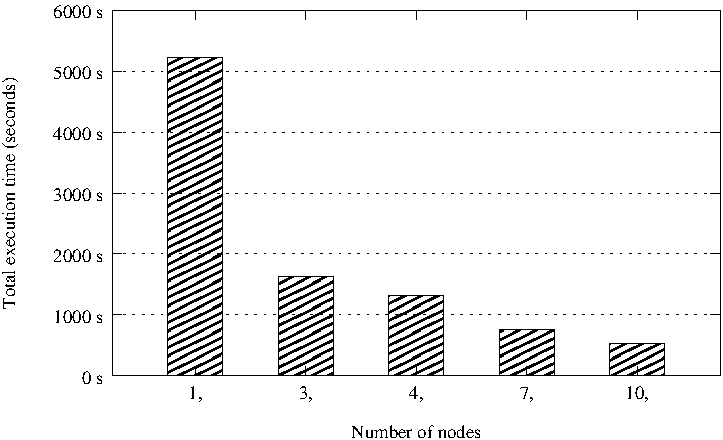
\includegraphics[width=0.80\textwidth]{img/hadoop/nodes-perf.pdf}
  \label{fig:nodes-pers-graph}
  \caption{Fragment of Web-UI interface displaying the progress of map tasks in the cluster consisting of 10 physical nodes, with one map slot each.}
\end{figure}

In order to summarise this section, one last observation should be made about Table \ref{table:more-nodes-results}, namely: in respect of adding more nodes to the Hadoop cluster, it seems that it scales nearly linear, as can be seen by comparing the number of nodes compared to the absolute speed-up, for example -- when running a cluster with \verb|10| nodes, the absolute speedup in relation to running on one node was \verb|9.87 times|, which is very near to a full 10. Thanks to this experiment one can conclude that (at least to such numbers of nodes) Hadoop is in fact \textit{nearly linearili scalable}, which is considered quite an achievement and would serve the growing-over-time needs of a data processing platform very well.


% ------------------------------------------------------------------------------------------
\subsection{Tuning cluster utilization through setting map / reduce slot numbers}
\label{sec:tuning-cluster-utilisation}
The last investigated option available for increasing cluster utilisation investigated was the \verb|mapred.map.tasks| setting and it's corresponding \verb|mapred.reduce.tasks|, as hinted by Eric Sammer in \cite{hadoop-ops}.

\begin{figure}[ch!]
  \centering
  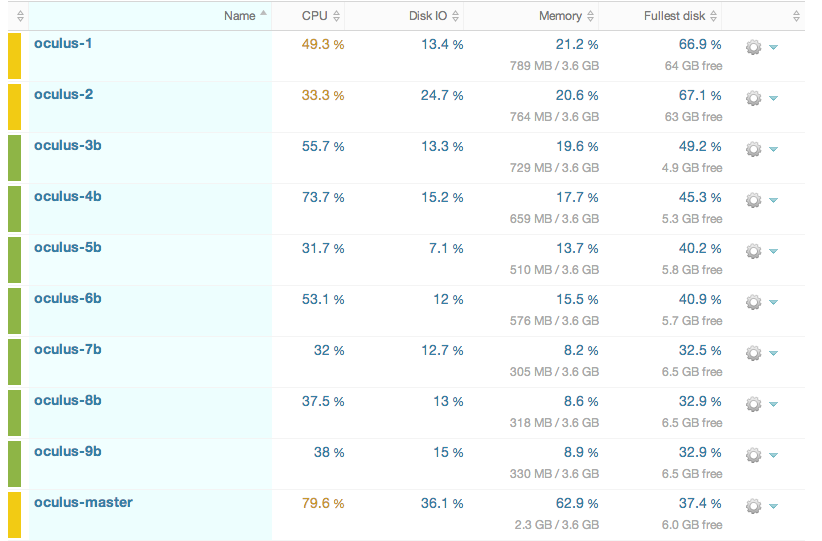
\includegraphics[width=0.8\textwidth]{img/hadoop/10nodes-newrelic-suffering-from-no-data-locallity}
  \label{fig:ten-under-utilised-cluster}
  \caption{An example of an underutilised cluster, where each node has 1 map and 1 reduce slot, yet the computed task is not draining the available CPU time, leading to wasting precious compute time.}
\end{figure}

These settings influence the number of Map and Reduce ''slots'' available for the scheduler on each node. By default these are set to 1 map task for each physical CPU available on the node (as can be seen on Figure \ref{fig:four-nodes-config}, where \textit{oculus-3-cpu} has 2 physical CPUs, and was automatically assigned 2 map and reduce slots). When running multiple example jobs on the cluster, it was discovered that some ''low utilisation'' jobs would needlessly occupy precious map slots on the cluster -- leading to such worst-case scenarios as depicted on Figure \ref{fig:ten-under-utilised-cluster}, where all nodes (all of which are of type: \textit{n1-standard-1 (1 vCPU, 3.8 GB memory)}) are processing one task and which occupies 100\% of their task slots (because each has 1 CPU), yet the task is \textit{not} CPU intensive, which leads to wasting precious CPU time. It would be much more efficient to allow these nodes to run at least 2 map and reduce tasks at the same time - since they they won't be competing for each other's CPU time.

\begin{figure}[ch!]
  \centering
  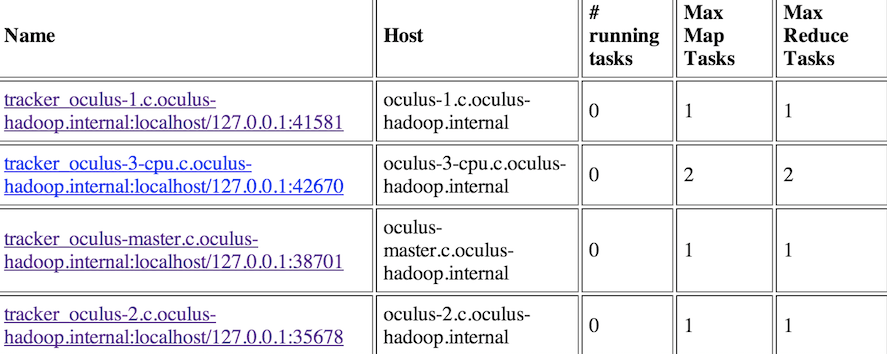
\includegraphics[width=\textwidth]{img/hadoop/4node-cluster-config}
  \label{fig:four-nodes-config}
  \caption{Fragment of Web-UI displaying the connected datanodes. The oculus-3 node is an high-cpu instance, and has more slots than the remaining nodes.}
\end{figure}

In order to avoid cluster under utilisation as seen on Figure \ref{fig:ten-under-utilised-cluster} (where 10 nodes are working, yet the vast majority of them only utilises around 30\% of their CPU), the number of concurrent tasks to be executed on one node was increased to 2 map and 2 reduce tasks. Literature recommends using \verb|rount(1.5 * nrOfCpus)| tasks per node, yet this setting should be always accustomed to the workload a cluster is expiriencing. Having this in mind, a scaled down cluster may actually be more efficient on processing such jobs. The changed configuration included 4 nodes, all of which were set-up fo host 2 map slots and 2 reduce slots. The CPU load on the cluster in such configuration, performing the same job as seen on Figure \ref{fig:four-nodes-config}, can be seen on Figure \ref{fig:cpu-load-during-job}.

\begin{figure}[ch!]
  \centering
  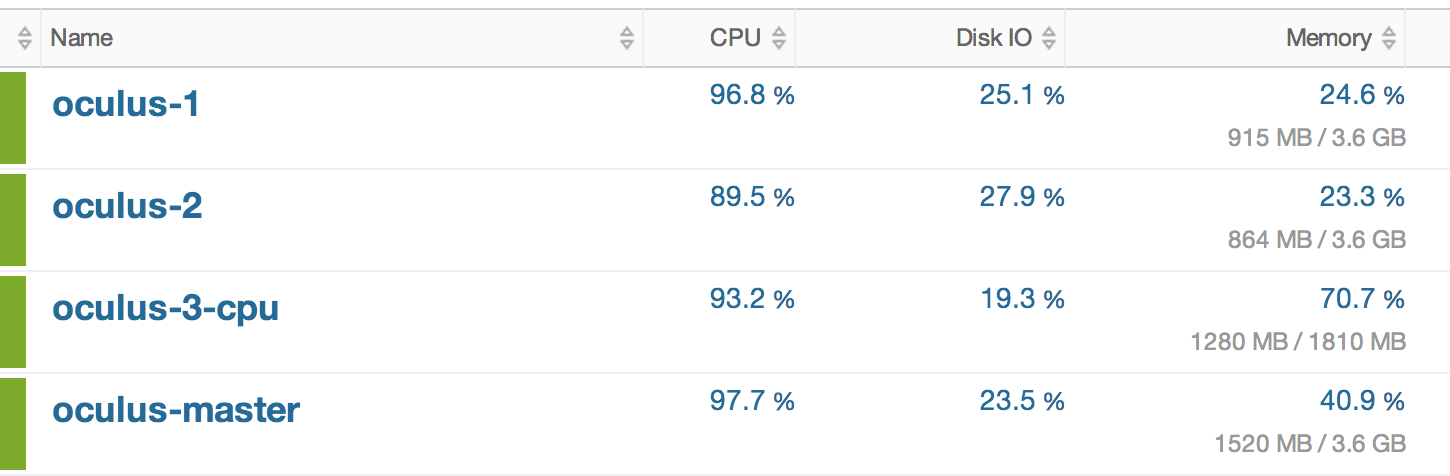
\includegraphics[width=\textwidth]{img/hadoop/monitoring-during-processing}
  \label{fig:cpu-load-during-job}
  \caption{Screenshot of New Relic (cluster monitoring software) displaying CPU and memory utilisation during the execution of an CPU intensive map reduce job.}
\end{figure}

It is worth keeping in mind that cost efficiency usually is also an important business need and simply adding more servers sometimes isn't an available option. Even more so, sometimes we may end up over provisioning servers -- as seen in Figure \ref{fig:ten-under-utilised-cluster}, so while simply adding more servers is very tempting and usually works very well on Hadoop clusters (as seen in Section \ref{sec:tuning-number-of-nodes}), one should always first try to fine tune the cluster to the specific work-load it is experiencing. In the case shown in this section, a fine-tuned 4 node cluster was able to perform almost as good (for this set of jobs), as the under utilised 10 node cluster. In real life clusters will always execute very different workloads at the same time, so it may be very hard to fine tune it for very percise scenarios, yet the effort of changing configurations of cluster members can sometimes prevent the need of adding more servers, so it should be always considered first -- unless a long term cluster expansion (e.g. ''adding 100 nodes, in the next 2 months'') is planned directly.

% ------------------------------------------------------------------------------------------------------------------------------------------------
%\section{Denormalisation as way to increase lookup performance in the Analyser's HBase interactions}
%\label{sec:optimising-hbase}
%
%While all performance optimisations mentioned in the Section about Hadoop scaling, directly impact HBase performance



% ------------------------------------------------------------------------------------------------------------------------------------------------
\section{Scaling out the Loader's Akka Cluster}
\label{sec:scaling-akka}

Scaling the Loader sub-system in this project was not very challanging because of the Actor System provided by Akka being so efficient where as the tasks performed by a node once it got a ''download movie'' message being measured in multiple minutes (up to 10 minutes for long movies -- since most creative commons licensed movies are not very long).

\subsection{Scaling out by adding more nodes}
\label{sec:scaling-akka-out}

The one optimization performed during this work was distributing ''download'' tasks to different nodes, so that two nodes in the cluster would download movies and upload the raw data into HDFS, for later processing by the Hadoop Map Reduce Jobs. By being mostly responsible for downloading, and uploading large files from YouTube and into HDFS, and only the minority of time being spent on crawling YouTube for additional movies to download scaling out the Loader was not a priority in boosting the overall systems performance.

Nevertheless, using Akka's clustering module it was possible to easily scale out the cluster and add new nodes to it, \textit{without the need of stopping the cluster}. The strategy was to deploy one downloader on each of the nodes, and make the node join the Akka cluster. Other nodes in the system would be notified that a new node has joined and can ask it to perform work. A full example of this workflow is presented in Listing \ref{lst:scaling-akka-cluster}, where the \verb|YoutubeCrawlActor| is configured to listen for cluster membership changes (on line 6), and then can react on members joining and leaving (lines 14 and 15) by adding and removing them from the RoundRobinRouter (which was explained in detail in Section \ref{sec:loader-basics}. Then, upon parsing a website and extracting links from it, the Router can be used to evenly distribute work among the registered downlaoder actors (lines 11 and 12).


\begin{lstlisting}[caption={Listening for Cluster events in Akka allows the application to dynamically respond to nodes being added to the cluster, and spreading the load in application logic to other nodes.}, label={lst:scaling-akka-cluster}]
class YoutubeCrawlActor extends Actor with OculusSelections {
  val cluster = Cluster(context.system)

  val downloadersRouter = Router(RoundRobinRoutingLogic())

  override def preStart() = cluster.subscribe(self, classOf[MemberEvent])
  override def postStop() = cluster.unsubscribe(self)

  def receive = {
    case CrawlYoutubePage(url) =>
      val urls = extractVideoUrls(fetchPage(url))
      urls foreach { downloadersRouter ! DownloadFromYoutube(_) }

    case MemberUp(m) => 
      downloadersRouter addRoutee downloaderSelection(m)
    
    case MemberDown(m) => 
      downloadersRouter removeRoutee downloaderSelection(m)
  }
}
\end{lstlisting}

Using Akka's clustering module in the Loader allows the system to scale dynamically, without ever needing to be turned off -- an important thing in long running distributed systems. The system turned out to be hard to measure accurately, due to the many moving parts (such as queue build up, non-determinism of which node would join at what time, and which video it would be assigned to download), yet generally speaking adding one more node would simply add one processing slot for the Download action -- similarily as in the Hadoop scenario adding a node would.

Akka by itself does not provide simple tracking of message and it's results, which is inherently a hard problem to solve, since one would have to track each message's ''parent''. Akka is a rather low level tool, whereas Hadoop is a dedicated platform for tracking progress od Jobs in distributed systems -- thus the conclusion is that it is easier to reason formally about a pure Actor systems behavior, than it is to strictly measure it (as least at the level of complication this problem is representing). Having this said, such monitoring would have to be built into the Oculus system, and is not provided by Akka itself -- sadly this feature was not implemented in the reference system, and remains an open problem, as well as field of intensive research -- as can be seen in multiple open source projects trying to solve this problem, such as Kamon \cite{kamon} or akka-tracing \cite{akka-tracing}.

Summarising Akka's scalability -- as communication is done directly between two nodes after they have joined the Cluster, the overhead of communication is very low (as low as serializing a message and sending it over-the-wise). This also means that adding new nodes should have improved the system's performance in a nearly linear fashion, since the critical execution (slowest tasks) are executed in an ''one Downloader per node'' fashion, and these tasks consume the complete available memory and CPU limits given to JVMs running this application. Tracing the exact performance impact for such complex message flows however, proved to be non trivial and has not been implemented as part of this thesis.



% ------------------------------------------------------------------------------------------------------------------------------------------------
\section{Summary of scaling methods}
\label{sec:scaling-summary}

In this chapter we have seen multiple methods to scale distributed systems and encountered both gains and problems while doing so.

Both systems (the Loader, as well as the Analyser) were able to \textit{scale-out} in a nearly linear fashion, although observing this exact change proved to be non trivial in the purely Akka based system. This is because Akka is rather meant to be as building block for systems such as Hadoop, and comparing them directly on this matter may seem unfair -- as in comparing a tool to a car, built using tools. One should remember this when selecting to either ''use'' or ''implement'' an distributed computation platform, and take into account that using some solutions the monitoring already comes built in -- as in the very old Hadoop eco-system -- and sometimes it does not (yet), as is currently the case with pure akka applications.

The ease of scaling out both systems was really impressive, yet in the case of Hadoop one has to directly tell the master-node via configuration changes about the new slave node joining the cluster, as explained in Section \ref{sec:growing-the-cluster} (''Growing the Cluster''). This is an inherent design flaw in Hadoop systems, since they always have one master node (although recent versions try to go away from this centralised topology). Akka on the other hand, with it's \textit{masterless cluster} is able to join nodes automatically, if they get in contact with any node that is already part of the cluster. Here we can see Akka's clustering mechanisms being superior yet \textit{less specialised} than the Hadoop one.

Summing up, both systems can be easily scaled up (by adding more powerful machines) or out (by adding more servers), and have displayed remarcable performance and stability throughout the tests conducted during this work. One should always remember that those two options should go in pair with each other, and that sometimes configuring the cluster in a better way may yield better results than blindy adding more nodes to the cluster. It is also crucial to have sophisticated monitoring installed in such cluster installations, as without them it would have been hard to detect and fix the cluster under-utilisation problem that was addressed in Section \ref{sec:tuning-cluster-utilisation}.



\chapter{Conclusions}
\label{chap:conclusions}

The primary goal of this thesis was to research distributed media processing. This has been achieved by implementing an reference system, which replicated the needs and workload of a quite realistic system that would have to analyse video data.

The implemented reference system was able to fulfil it's initial requirements of detecting ''near duplicate'' movies. Test runs using publicly available creative-commons licensed movies have been performed. The system was also tuned to perform in the face of maliciously modified video content (mirrored, blurred or otherwise distorted), and the system was still able to identify matching video data. Certain optimisations were applied to make the search times possibly fast. These optimisations required gaining knowledge about HBase's internals and designing a specialised row key, as has described in Chapter \ref{chap:analysis-examples}. On the perceptual hashing front there is still much work that could have been applied to the proposed system, and better fingerprinting methods could have been applied -- yes as this was not the primary focus of this thesis, the proposed system performed within it's expected expected performance boundaries of a few hours of processing per each movie.

This system was then used to perform multiple scalability tests and optimisations, as described in Chapter \ref{chap:perf-scalability}. The Hadoop cluster was first scaled horizontally by adding mode nodes and measuring it's performance improvement -- which turned out to be nearly linear, if one trades of storage duplication for computation speed, or sligtly lower if replication factors would not be tuned in accordance to the clusters size. The cluster had also undergon configuration as well as application level improvements aimed at utilising HDFS at it's best.

To conclude, the investigated distributed systems provide an astounding platform to work on. Akka as well as Hadoop and it's rich eco-system allow to easily build resilient and scalable applications which are able to process huge amounts of data. Hadoop especially confirmed it's ability to scale-out very easily, and has proven to be a very stable execution platform. The operational overhead of starting clusters that such applications require can be lessened by far thanks to using modern configuration provisioning utilities such as Chef, and public cloud providers make testing clusters in varying sizes very easy. In the forseeable future we will see more kinds of these tools being perfected, as the demand for applications of such scale is still growing.

\appendix
\chapter{Automated cluster deployment}
\label{app:chef}
This chapter describes the automated tooling which has been used during the implementation of the reference system mentioned in this thesis in order to drastically increase turnaround time during development as well as cluster scaling.

Due to the complexities of maintaining possibly hundreds of virtual machines with similar (or even identical) configurations the time it would take to provision, configure and deplot applications on each new server in the cluster would render this process very slow and fiesable. Instead, tools and platforms have been applied to simplify and speed-up the turnaround time when adding new servers to the cluster. 

In Section \ref{sec:automated-server-provisioning} the used cloud intrafstucture is introduced, along with a few examples of automating server provisioning using simple yet powerful command-line tools. 

In Section \ref{sec:automated-conf-provisioning} Opscode Chef -- the tool used to configure, as well as install dependencies and deploy applications is introduced.

\section{Automated server provisioning -- Google Compute Engine}
\label{sec:automated-server-provisioning}

In order to provision virtual machines for running the applicationc cluster Google's Compute Engine ''Infrastructure as a Service'' (also known under the acronym \textit{IAAS}) was used. 

Creating a new instance on GCE (\textit{Google Compute Engine}) can be done via an admin console under \verb|cloud.google.com| or using command line tooling (or plain JSON API calls). During this project the most used method was the command line API, as it is simple to prepare scripts for spinning up multiple VMs and combining this step with provisioning configuration to them using Chef (which will be explained in Section \ref{sec:automated-conf-provisioning}. An example of how a new instance on GCE can be started is illustrated on Listing \ref{lst:new-gce-instance-bash}.

\begin{lstlisting}[caption={Creating new instance on GCE}, label={lst:new-gce-instance-bash}]
gcutil --service_version="v1" --project="oculus-hadoop" 
  addinstance "oculus-3" --machine_type="n1-standard-1" 
  --zone="us-central1-a" --tags="hadoop,datanode"
  --disk="large-4,deviceName=large-4,mode=READ_WRITE"
  --network="default" --external_ip_address="ephemeral" 
  --service_account_scopes="https://www.googleapis.com/auth/..." 
  --image="https://www.googleapis.com/.../images/debian-7-wheezy-v20140408" 
  --persistent_boot_disk="true" --auto_delete_boot_disk="true"
\end{lstlisting}


Listing \ref{lst:gcutil-list} shows the current cluster's status.

\todo{listing needs label}

\label{lst:gcutil-list}
\begin{verbatim}
# gcutil listinstances

+---------------+---------------+---------+------------+------------+
| name          | zone          | status  | network-ip | pub-ip     |
+---------------+---------------+---------+------------+------------+
| oculus-1      | us-central1-a | RUNNING | 10.240.x.x | 23.236.x.x |
+---------------+---------------+---------+------------+------------+
| oculus-2      | us-central1-a | RUNNING | 10.240.x.x | 108.59.x.x |
+---------------+---------------+---------+------------+------------+
| oculus-master | us-central1-a | RUNNING | 10.240.x.x | 108.59.x.x |
+---------------+---------------+---------+------------+------------+
\end{verbatim}

It it also possibe to invoke typical compute engine tasks using it's Chef (which is described in detail in Section \ref{sec:automated-conf-provisioning}) plugins, so that an it's even easier to use and investigate the running cluster:

\begin{verbatim}
# knife google server list --gce-zone us-central1-a

name           type           public ip  disks        zone           
oculus-1       n1-standard-1  23.x.x.x   d-1,large-4  us-central1-a  
oculus-2       n1-standard-1  23.x.x.x   d-2,large-1  us-central1-a  
oculus-master  n1-standard-1  23.x.x.x   m-0,large-3  us-central1-a  
\end{verbatim}


\label{sec:automated-conf-provisioning}
\section{Automated configuration and deployment -- Opscode Chef}

Chef is a tool which enables to easily manage configuration and deployment of services and apps across cloud infrastructure. It consists of a set of tools using which one can describe a servers configurational requirements, such as what services it should have installed. It provides multiple ways to execute the provisioning step yet for the sake of this thesis the simplest ''solo'' mode was used. 

When using Chef in solo mode, one prepares a specific ''$run\_list$'' that consists of names of cookbooks (which are simply a series of ''steps to execute'' in order to provision something) that should be applied to a given server, and then applying this ''$run\_list$'' to a given server. An example node file is shown on Listing \ref{lst:node}.

\begin{lstlisting}[caption={Example data-node.json file}]
{
  "run_list": [
    "role[base]",
    "role[datanode]"
  ]
}
\end{lstlisting}

A node description in turn relies on certain roles and recipes. Roles are defined as a list of recipes and properties that can be required together. The datanode role is fairly simple as seen on Listing \ref{lst:datanode-list}

\begin{lstlisting}[caption={Example roles/datanode.rb file}]
run_list "recipe[hadoop::datanode]"
\end{lstlisting}



\begin{lstlisting}[caption={Preparing and Cooking a server with in order to prepare it for becoming a Hadoop data-node},label={lst:cheffing-data-node}]
# knife solo prepare kmalawski@108.59.81.222 nodes/datanode.json
...
(Reading database ... 42465 files and directories currently installed.)
Preparing to replace chef 11.8.2-1.debian.6.0.5 (using .../chef_11.12.2-1_amd64.deb) ...
Unpacking replacement chef ...
Setting up chef (11.12.2-1) ...

# knife solo cook kmalawski@108.59.81.222 nodes/data-node.json
Uploading the kitchen...

\end{lstlisting}















\nocite{*}
\bibliography{bibliography}{}
\bibliographystyle{alpha}


\end{document}
